% Options for packages loaded elsewhere
\PassOptionsToPackage{unicode}{hyperref}
\PassOptionsToPackage{hyphens}{url}
%
\documentclass[
  10pt, ]{article}
\usepackage{lmodern}
\usepackage{amssymb,amsmath}
\usepackage{ifxetex,ifluatex}
\ifnum 0\ifxetex 1\fi\ifluatex 1\fi=0 % if pdftex
  \usepackage[T1]{fontenc}
  \usepackage[utf8]{inputenc}
  \usepackage{textcomp} % provide euro and other symbols
\else % if luatex or xetex
  \usepackage{unicode-math}
  \defaultfontfeatures{Scale=MatchLowercase}
  \defaultfontfeatures[\rmfamily]{Ligatures=TeX,Scale=1}
\fi
% Use upquote if available, for straight quotes in verbatim environments
\IfFileExists{upquote.sty}{\usepackage{upquote}}{}
\IfFileExists{microtype.sty}{% use microtype if available
  \usepackage[]{microtype}
  \UseMicrotypeSet[protrusion]{basicmath} % disable protrusion for tt fonts
}{}
\makeatletter
\@ifundefined{KOMAClassName}{% if non-KOMA class
  \IfFileExists{parskip.sty}{%
    \usepackage{parskip}
  }{% else
    \setlength{\parindent}{0pt}
    \setlength{\parskip}{6pt plus 2pt minus 1pt}}
}{% if KOMA class
  \KOMAoptions{parskip=half}}
\makeatother
\usepackage{xcolor}
\IfFileExists{xurl.sty}{\usepackage{xurl}}{} % add URL line breaks if available
\IfFileExists{bookmark.sty}{\usepackage{bookmark}}{\usepackage{hyperref}}
\hypersetup{
  hidelinks, pdfcreator={LaTeX via pandoc}}
\urlstyle{same} % disable monospaced font for URLs
\usepackage[margin=1.8cm]{geometry}
\usepackage{longtable,booktabs}
% Correct order of tables after \paragraph or \subparagraph
\usepackage{etoolbox}
\makeatletter
\patchcmd\longtable{\par}{\if@noskipsec\mbox{}\fi\par}{}{}
\makeatother
% Allow footnotes in longtable head/foot
\IfFileExists{footnotehyper.sty}{\usepackage{footnotehyper}}{\usepackage{footnote}}
\makesavenoteenv{longtable}
\usepackage{graphicx}
\makeatletter
\def\maxwidth{\ifdim\Gin@nat@width>\linewidth\linewidth\else\Gin@nat@width\fi}
\def\maxheight{\ifdim\Gin@nat@height>\textheight\textheight\else\Gin@nat@height\fi}
\makeatother
% Scale images if necessary, so that they will not overflow the page
% margins by default, and it is still possible to overwrite the defaults
% using explicit options in \includegraphics[width, height, ...]{}
\setkeys{Gin}{width=\maxwidth,height=\maxheight,keepaspectratio}
% Set default figure placement to htbp
\makeatletter
\def\fps@figure{htbp}
\makeatother
\setlength{\emergencystretch}{3em} % prevent overfull lines
\providecommand{\tightlist}{%
  \setlength{\itemsep}{0pt}\setlength{\parskip}{0pt}}
\setcounter{secnumdepth}{-\maxdimen} % remove section numbering
\usepackage{float}\floatplacement{figure}{H}

\author{}
\date{}

\begin{document}

\hypertarget{model-evaluation-ml-based-traffic-speed-prediction}{%
\section{Model Evaluation --- ML-Based Traffic Speed
Prediction}\label{model-evaluation-ml-based-traffic-speed-prediction}}

This document describes the evaluation of the trained models published in this repository, accompanying the paper ``Cloud-Fog-Edge Deployment of ML-Based Traffic Speed Prediction: An Empirical Analysis of Performance, Cost, and Scalability''.

\hypertarget{models}{%
\subsection{Models}\label{models}}

One multilayer perceptron per sensor direction (37 sensor directions; layer sizes 96-256-256-96-256, ReLU with dropout, \textasciitilde142k parameters, RMSprop optimiser, MSE loss, float32). Each model ships with its fitted input (x) and output (y) RobustScaler as \texttt{.pkl} files. Two model sets are published:

\begin{itemize}
\tightlist
\item
  \texttt{trained\_models\_full42y/} - the baseline models evaluated from the full-span (4.2-year) cold-start training regime on a fog computing platform: trained from 1 December 2020 to 1 February 2025 with the final 20\% held out; this model is used in the cold-start rows of the paper's Table 13 results.
\item
  \texttt{trained\_models\_base3y/} - the base 3-year trained model is also included so the paper's warm-start re-training experiments are reproducible.
\end{itemize}

All models use 15 engineered features (cyclic time encodings and event flags) from five-minute average-speed records of Greater Manchester drakewell sensors.

\hypertarget{evaluation-protocol}{%
\subsection{Evaluation protocol}\label{evaluation-protocol}}

The baseline model results come from the full-span (4.2-year) cold-start training regime reported in the paper. Each sensor's data is split chronologically 80/20; the final 20\% of the full span serves as the held-out test set - approximately April 2024 to February 2025, with the exact boundary varying per sensor between late January and late April 2024 depending on data completeness. Metrics are mean absolute error (MAE, mph), root mean squared error (RMSE, mph), and mean absolute percentage error (MAPE, \%). For a wider context, each row also reports the coefficient of variation of speed over the full modelled span, 1 December 2020 to 1 February 2025 (Speed CoV, dimensionless) - i.e., the variability of exactly the data the model was trained and evaluated on; the congestion frequency (share of five-minute intervals below 50\% of the sensor's 85th-percentile free-flow speed, over the full span). A complementary common-test-set evaluation (identical held-out periods for all re-training scenarios) is also summarised in the last section.

\hypertarget{per-sensor-results-full span data (cold-start 4.2-year-training-regime)}{%
\subsection{Per-sensor-results --- full span data (cold-start 4.2-year-training-regime)}\label{per-sensor-results-4.2-year-training-regime}}

All rows come from the published models in
\texttt{trained\_models\_full42y/}; their
all-sensor aggregate (bottom row) matches the cold-start cells of the paper's Table 13 cold-start full-tier model accuracy (11.98--11.99\%). Sensor directions with MAPE above 15\% are highlighted in bold.

\begin{longtable}[]{@{}lllllllll@{}}
\toprule
\begin{minipage}[b]{0.08\columnwidth}\raggedright
\#\strut
\end{minipage} & \begin{minipage}[b]{0.08\columnwidth}\raggedright
Tier group\strut
\end{minipage} & \begin{minipage}[b]{0.08\columnwidth}\raggedright
Sensor\strut
\end{minipage} & \begin{minipage}[b]{0.08\columnwidth}\raggedright
MAE (mph)\strut
\end{minipage} & \begin{minipage}[b]{0.08\columnwidth}\raggedright
RMSE (mph)\strut
\end{minipage} & \begin{minipage}[b]{0.08\columnwidth}\raggedright
MAPE (\%)\strut
\end{minipage} & \begin{minipage}[b]{0.08\columnwidth}\raggedright
Speed CoV\strut
\end{minipage} & \begin{minipage}[b]{0.08\columnwidth}\raggedright
Congestion (\%)\strut
\end{minipage} & \begin{minipage}[b]{0.08\columnwidth}\raggedright
Test samples\strut
\end{minipage}\tabularnewline
\midrule
\endhead
\begin{minipage}[t]{0.08\columnwidth}\raggedright
1\strut
\end{minipage} & \begin{minipage}[t]{0.08\columnwidth}\raggedright
tiny\strut
\end{minipage} & \begin{minipage}[t]{0.08\columnwidth}\raggedright
1163 nw\strut
\end{minipage} & \begin{minipage}[t]{0.08\columnwidth}\raggedright
2.85\strut
\end{minipage} & \begin{minipage}[t]{0.08\columnwidth}\raggedright
4.18\strut
\end{minipage} & \begin{minipage}[t]{0.08\columnwidth}\raggedright
12.51\strut
\end{minipage} & \begin{minipage}[t]{0.08\columnwidth}\raggedright
0.162\strut
\end{minipage} & \begin{minipage}[t]{0.08\columnwidth}\raggedright
1.31\strut
\end{minipage} & \begin{minipage}[t]{0.08\columnwidth}\raggedright
84,322\strut
\end{minipage}\tabularnewline
\begin{minipage}[t]{0.08\columnwidth}\raggedright
2\strut
\end{minipage} & \begin{minipage}[t]{0.08\columnwidth}\raggedright
small\strut
\end{minipage} & \begin{minipage}[t]{0.08\columnwidth}\raggedright
1071 ne\strut
\end{minipage} & \begin{minipage}[t]{0.08\columnwidth}\raggedright
2.26\strut
\end{minipage} & \begin{minipage}[t]{0.08\columnwidth}\raggedright
4.02\strut
\end{minipage} & \begin{minipage}[t]{0.08\columnwidth}\raggedright
12.53\strut
\end{minipage} & \begin{minipage}[t]{0.08\columnwidth}\raggedright
0.128\strut
\end{minipage} & \begin{minipage}[t]{0.08\columnwidth}\raggedright
1.72\strut
\end{minipage} & \begin{minipage}[t]{0.08\columnwidth}\raggedright
86,622\strut
\end{minipage}\tabularnewline
\begin{minipage}[t]{0.08\columnwidth}\raggedright
3\strut
\end{minipage} & \begin{minipage}[t]{0.08\columnwidth}\raggedright
small\strut
\end{minipage} & \begin{minipage}[t]{0.08\columnwidth}\raggedright
1071 sw\strut
\end{minipage} & \begin{minipage}[t]{0.08\columnwidth}\raggedright
1.40\strut
\end{minipage} & \begin{minipage}[t]{0.08\columnwidth}\raggedright
2.19\strut
\end{minipage} & \begin{minipage}[t]{0.08\columnwidth}\raggedright
5.00\strut
\end{minipage} & \begin{minipage}[t]{0.08\columnwidth}\raggedright
0.082\strut
\end{minipage} & \begin{minipage}[t]{0.08\columnwidth}\raggedright
0.17\strut
\end{minipage} & \begin{minipage}[t]{0.08\columnwidth}\raggedright
86,872\strut
\end{minipage}\tabularnewline
\begin{minipage}[t]{0.08\columnwidth}\raggedright
4\strut
\end{minipage} & \begin{minipage}[t]{0.08\columnwidth}\raggedright
small\strut
\end{minipage} & \begin{minipage}[t]{0.08\columnwidth}\raggedright
1407 n\strut
\end{minipage} & \begin{minipage}[t]{0.08\columnwidth}\raggedright
1.92\strut
\end{minipage} & \begin{minipage}[t]{0.08\columnwidth}\raggedright
2.95\strut
\end{minipage} & \begin{minipage}[t]{0.08\columnwidth}\raggedright
8.44\strut
\end{minipage} & \begin{minipage}[t]{0.08\columnwidth}\raggedright
0.129\strut
\end{minipage} & \begin{minipage}[t]{0.08\columnwidth}\raggedright
1.15\strut
\end{minipage} & \begin{minipage}[t]{0.08\columnwidth}\raggedright
87,024\strut
\end{minipage}\tabularnewline
\begin{minipage}[t]{0.08\columnwidth}\raggedright
5\strut
\end{minipage} & \begin{minipage}[t]{0.08\columnwidth}\raggedright
small\strut
\end{minipage} & \begin{minipage}[t]{0.08\columnwidth}\raggedright
1407 s\strut
\end{minipage} & \begin{minipage}[t]{0.08\columnwidth}\raggedright
2.08\strut
\end{minipage} & \begin{minipage}[t]{0.08\columnwidth}\raggedright
3.12\strut
\end{minipage} & \begin{minipage}[t]{0.08\columnwidth}\raggedright
10.08\strut
\end{minipage} & \begin{minipage}[t]{0.08\columnwidth}\raggedright
0.171\strut
\end{minipage} & \begin{minipage}[t]{0.08\columnwidth}\raggedright
3.80\strut
\end{minipage} & \begin{minipage}[t]{0.08\columnwidth}\raggedright
86,909\strut
\end{minipage}\tabularnewline
\begin{minipage}[t]{0.08\columnwidth}\raggedright
6\strut
\end{minipage} & \begin{minipage}[t]{0.08\columnwidth}\raggedright
small\strut
\end{minipage} & \begin{minipage}[t]{0.08\columnwidth}\raggedright
1417 s\strut
\end{minipage} & \begin{minipage}[t]{0.08\columnwidth}\raggedright
1.43\strut
\end{minipage} & \begin{minipage}[t]{0.08\columnwidth}\raggedright
1.99\strut
\end{minipage} & \begin{minipage}[t]{0.08\columnwidth}\raggedright
6.89\strut
\end{minipage} & \begin{minipage}[t]{0.08\columnwidth}\raggedright
0.111\strut
\end{minipage} & \begin{minipage}[t]{0.08\columnwidth}\raggedright
0.20\strut
\end{minipage} & \begin{minipage}[t]{0.08\columnwidth}\raggedright
86,699\strut
\end{minipage}\tabularnewline
\begin{minipage}[t]{0.08\columnwidth}\raggedright
7\strut
\end{minipage} & \begin{minipage}[t]{0.08\columnwidth}\raggedright
small\strut
\end{minipage} & \begin{minipage}[t]{0.08\columnwidth}\raggedright
1420 nw\strut
\end{minipage} & \begin{minipage}[t]{0.08\columnwidth}\raggedright
1.92\strut
\end{minipage} & \begin{minipage}[t]{0.08\columnwidth}\raggedright
3.08\strut
\end{minipage} & \begin{minipage}[t]{0.08\columnwidth}\raggedright
10.46\strut
\end{minipage} & \begin{minipage}[t]{0.08\columnwidth}\raggedright
0.158\strut
\end{minipage} & \begin{minipage}[t]{0.08\columnwidth}\raggedright
3.37\strut
\end{minipage} & \begin{minipage}[t]{0.08\columnwidth}\raggedright
86,446\strut
\end{minipage}\tabularnewline
\begin{minipage}[t]{0.08\columnwidth}\raggedright
8\strut
\end{minipage} & \begin{minipage}[t]{0.08\columnwidth}\raggedright
small\strut
\end{minipage} & \begin{minipage}[t]{0.08\columnwidth}\raggedright
1425 e\strut
\end{minipage} & \begin{minipage}[t]{0.08\columnwidth}\raggedright
2.04\strut
\end{minipage} & \begin{minipage}[t]{0.08\columnwidth}\raggedright
3.54\strut
\end{minipage} & \begin{minipage}[t]{0.08\columnwidth}\raggedright
4.51\strut
\end{minipage} & \begin{minipage}[t]{0.08\columnwidth}\raggedright
0.066\strut
\end{minipage} & \begin{minipage}[t]{0.08\columnwidth}\raggedright
0.14\strut
\end{minipage} & \begin{minipage}[t]{0.08\columnwidth}\raggedright
86,582\strut
\end{minipage}\tabularnewline
\begin{minipage}[t]{0.08\columnwidth}\raggedright
9\strut
\end{minipage} & \begin{minipage}[t]{0.08\columnwidth}\raggedright
small\strut
\end{minipage} & \begin{minipage}[t]{0.08\columnwidth}\raggedright
1425 w\strut
\end{minipage} & \begin{minipage}[t]{0.08\columnwidth}\raggedright
2.53\strut
\end{minipage} & \begin{minipage}[t]{0.08\columnwidth}\raggedright
5.08\strut
\end{minipage} & \begin{minipage}[t]{0.08\columnwidth}\raggedright
8.29\strut
\end{minipage} & \begin{minipage}[t]{0.08\columnwidth}\raggedright
0.080\strut
\end{minipage} & \begin{minipage}[t]{0.08\columnwidth}\raggedright
0.51\strut
\end{minipage} & \begin{minipage}[t]{0.08\columnwidth}\raggedright
86,589\strut
\end{minipage}\tabularnewline
\begin{minipage}[t]{0.08\columnwidth}\raggedright
10\strut
\end{minipage} & \begin{minipage}[t]{0.08\columnwidth}\raggedright
small\strut
\end{minipage} & \begin{minipage}[t]{0.08\columnwidth}\raggedright
\textbf{1426 w}\strut
\end{minipage} & \begin{minipage}[t]{0.08\columnwidth}\raggedright
4.13\strut
\end{minipage} & \begin{minipage}[t]{0.08\columnwidth}\raggedright
7.70\strut
\end{minipage} & \begin{minipage}[t]{0.08\columnwidth}\raggedright
\textbf{19.92}\strut
\end{minipage} & \begin{minipage}[t]{0.08\columnwidth}\raggedright
0.171\strut
\end{minipage} & \begin{minipage}[t]{0.08\columnwidth}\raggedright
3.26\strut
\end{minipage} & \begin{minipage}[t]{0.08\columnwidth}\raggedright
87,203\strut
\end{minipage}\tabularnewline
\begin{minipage}[t]{0.08\columnwidth}\raggedright
11\strut
\end{minipage} & \begin{minipage}[t]{0.08\columnwidth}\raggedright
medium\strut
\end{minipage} & \begin{minipage}[t]{0.08\columnwidth}\raggedright
1020 nw\strut
\end{minipage} & \begin{minipage}[t]{0.08\columnwidth}\raggedright
2.04\strut
\end{minipage} & \begin{minipage}[t]{0.08\columnwidth}\raggedright
2.94\strut
\end{minipage} & \begin{minipage}[t]{0.08\columnwidth}\raggedright
8.18\strut
\end{minipage} & \begin{minipage}[t]{0.08\columnwidth}\raggedright
0.128\strut
\end{minipage} & \begin{minipage}[t]{0.08\columnwidth}\raggedright
0.63\strut
\end{minipage} & \begin{minipage}[t]{0.08\columnwidth}\raggedright
85,096\strut
\end{minipage}\tabularnewline
\begin{minipage}[t]{0.08\columnwidth}\raggedright
12\strut
\end{minipage} & \begin{minipage}[t]{0.08\columnwidth}\raggedright
medium\strut
\end{minipage} & \begin{minipage}[t]{0.08\columnwidth}\raggedright
1020 se\strut
\end{minipage} & \begin{minipage}[t]{0.08\columnwidth}\raggedright
1.75\strut
\end{minipage} & \begin{minipage}[t]{0.08\columnwidth}\raggedright
2.52\strut
\end{minipage} & \begin{minipage}[t]{0.08\columnwidth}\raggedright
7.03\strut
\end{minipage} & \begin{minipage}[t]{0.08\columnwidth}\raggedright
0.139\strut
\end{minipage} & \begin{minipage}[t]{0.08\columnwidth}\raggedright
0.41\strut
\end{minipage} & \begin{minipage}[t]{0.08\columnwidth}\raggedright
84,978\strut
\end{minipage}\tabularnewline
\begin{minipage}[t]{0.08\columnwidth}\raggedright
13\strut
\end{minipage} & \begin{minipage}[t]{0.08\columnwidth}\raggedright
medium\strut
\end{minipage} & \begin{minipage}[t]{0.08\columnwidth}\raggedright
1056 e\strut
\end{minipage} & \begin{minipage}[t]{0.08\columnwidth}\raggedright
1.29\strut
\end{minipage} & \begin{minipage}[t]{0.08\columnwidth}\raggedright
1.81\strut
\end{minipage} & \begin{minipage}[t]{0.08\columnwidth}\raggedright
5.66\strut
\end{minipage} & \begin{minipage}[t]{0.08\columnwidth}\raggedright
0.086\strut
\end{minipage} & \begin{minipage}[t]{0.08\columnwidth}\raggedright
0.11\strut
\end{minipage} & \begin{minipage}[t]{0.08\columnwidth}\raggedright
83,327\strut
\end{minipage}\tabularnewline
\begin{minipage}[t]{0.08\columnwidth}\raggedright
14\strut
\end{minipage} & \begin{minipage}[t]{0.08\columnwidth}\raggedright
medium\strut
\end{minipage} & \begin{minipage}[t]{0.08\columnwidth}\raggedright
1056 w\strut
\end{minipage} & \begin{minipage}[t]{0.08\columnwidth}\raggedright
1.39\strut
\end{minipage} & \begin{minipage}[t]{0.08\columnwidth}\raggedright
2.08\strut
\end{minipage} & \begin{minipage}[t]{0.08\columnwidth}\raggedright
6.28\strut
\end{minipage} & \begin{minipage}[t]{0.08\columnwidth}\raggedright
0.099\strut
\end{minipage} & \begin{minipage}[t]{0.08\columnwidth}\raggedright
0.17\strut
\end{minipage} & \begin{minipage}[t]{0.08\columnwidth}\raggedright
84,435\strut
\end{minipage}\tabularnewline
\begin{minipage}[t]{0.08\columnwidth}\raggedright
15\strut
\end{minipage} & \begin{minipage}[t]{0.08\columnwidth}\raggedright
medium\strut
\end{minipage} & \begin{minipage}[t]{0.08\columnwidth}\raggedright
1063 e\strut
\end{minipage} & \begin{minipage}[t]{0.08\columnwidth}\raggedright
1.44\strut
\end{minipage} & \begin{minipage}[t]{0.08\columnwidth}\raggedright
2.34\strut
\end{minipage} & \begin{minipage}[t]{0.08\columnwidth}\raggedright
5.41\strut
\end{minipage} & \begin{minipage}[t]{0.08\columnwidth}\raggedright
0.097\strut
\end{minipage} & \begin{minipage}[t]{0.08\columnwidth}\raggedright
0.43\strut
\end{minipage} & \begin{minipage}[t]{0.08\columnwidth}\raggedright
84,066\strut
\end{minipage}\tabularnewline
\begin{minipage}[t]{0.08\columnwidth}\raggedright
16\strut
\end{minipage} & \begin{minipage}[t]{0.08\columnwidth}\raggedright
medium\strut
\end{minipage} & \begin{minipage}[t]{0.08\columnwidth}\raggedright
1063 w\strut
\end{minipage} & \begin{minipage}[t]{0.08\columnwidth}\raggedright
1.58\strut
\end{minipage} & \begin{minipage}[t]{0.08\columnwidth}\raggedright
2.34\strut
\end{minipage} & \begin{minipage}[t]{0.08\columnwidth}\raggedright
5.29\strut
\end{minipage} & \begin{minipage}[t]{0.08\columnwidth}\raggedright
0.110\strut
\end{minipage} & \begin{minipage}[t]{0.08\columnwidth}\raggedright
0.52\strut
\end{minipage} & \begin{minipage}[t]{0.08\columnwidth}\raggedright
84,086\strut
\end{minipage}\tabularnewline
\begin{minipage}[t]{0.08\columnwidth}\raggedright
17\strut
\end{minipage} & \begin{minipage}[t]{0.08\columnwidth}\raggedright
medium\strut
\end{minipage} & \begin{minipage}[t]{0.08\columnwidth}\raggedright
\textbf{1163 se}\strut
\end{minipage} & \begin{minipage}[t]{0.08\columnwidth}\raggedright
2.95\strut
\end{minipage} & \begin{minipage}[t]{0.08\columnwidth}\raggedright
4.70\strut
\end{minipage} & \begin{minipage}[t]{0.08\columnwidth}\raggedright
\textbf{16.91}\strut
\end{minipage} & \begin{minipage}[t]{0.08\columnwidth}\raggedright
0.190\strut
\end{minipage} & \begin{minipage}[t]{0.08\columnwidth}\raggedright
5.41\strut
\end{minipage} & \begin{minipage}[t]{0.08\columnwidth}\raggedright
84,329\strut
\end{minipage}\tabularnewline
\begin{minipage}[t]{0.08\columnwidth}\raggedright
18\strut
\end{minipage} & \begin{minipage}[t]{0.08\columnwidth}\raggedright
medium\strut
\end{minipage} & \begin{minipage}[t]{0.08\columnwidth}\raggedright
1165 se\strut
\end{minipage} & \begin{minipage}[t]{0.08\columnwidth}\raggedright
2.11\strut
\end{minipage} & \begin{minipage}[t]{0.08\columnwidth}\raggedright
3.32\strut
\end{minipage} & \begin{minipage}[t]{0.08\columnwidth}\raggedright
9.27\strut
\end{minipage} & \begin{minipage}[t]{0.08\columnwidth}\raggedright
0.130\strut
\end{minipage} & \begin{minipage}[t]{0.08\columnwidth}\raggedright
1.93\strut
\end{minipage} & \begin{minipage}[t]{0.08\columnwidth}\raggedright
85,811\strut
\end{minipage}\tabularnewline
\begin{minipage}[t]{0.08\columnwidth}\raggedright
19\strut
\end{minipage} & \begin{minipage}[t]{0.08\columnwidth}\raggedright
medium\strut
\end{minipage} & \begin{minipage}[t]{0.08\columnwidth}\raggedright
\textbf{1404 e}\strut
\end{minipage} & \begin{minipage}[t]{0.08\columnwidth}\raggedright
5.46\strut
\end{minipage} & \begin{minipage}[t]{0.08\columnwidth}\raggedright
8.86\strut
\end{minipage} & \begin{minipage}[t]{0.08\columnwidth}\raggedright
\textbf{42.45}\strut
\end{minipage} & \begin{minipage}[t]{0.08\columnwidth}\raggedright
0.201\strut
\end{minipage} & \begin{minipage}[t]{0.08\columnwidth}\raggedright
6.28\strut
\end{minipage} & \begin{minipage}[t]{0.08\columnwidth}\raggedright
83,741\strut
\end{minipage}\tabularnewline
\begin{minipage}[t]{0.08\columnwidth}\raggedright
20\strut
\end{minipage} & \begin{minipage}[t]{0.08\columnwidth}\raggedright
medium\strut
\end{minipage} & \begin{minipage}[t]{0.08\columnwidth}\raggedright
1413 ne\strut
\end{minipage} & \begin{minipage}[t]{0.08\columnwidth}\raggedright
1.51\strut
\end{minipage} & \begin{minipage}[t]{0.08\columnwidth}\raggedright
2.15\strut
\end{minipage} & \begin{minipage}[t]{0.08\columnwidth}\raggedright
6.01\strut
\end{minipage} & \begin{minipage}[t]{0.08\columnwidth}\raggedright
0.102\strut
\end{minipage} & \begin{minipage}[t]{0.08\columnwidth}\raggedright
0.34\strut
\end{minipage} & \begin{minipage}[t]{0.08\columnwidth}\raggedright
85,531\strut
\end{minipage}\tabularnewline
\begin{minipage}[t]{0.08\columnwidth}\raggedright
21\strut
\end{minipage} & \begin{minipage}[t]{0.08\columnwidth}\raggedright
medium\strut
\end{minipage} & \begin{minipage}[t]{0.08\columnwidth}\raggedright
1413 sw\strut
\end{minipage} & \begin{minipage}[t]{0.08\columnwidth}\raggedright
1.73\strut
\end{minipage} & \begin{minipage}[t]{0.08\columnwidth}\raggedright
2.41\strut
\end{minipage} & \begin{minipage}[t]{0.08\columnwidth}\raggedright
6.91\strut
\end{minipage} & \begin{minipage}[t]{0.08\columnwidth}\raggedright
0.100\strut
\end{minipage} & \begin{minipage}[t]{0.08\columnwidth}\raggedright
0.11\strut
\end{minipage} & \begin{minipage}[t]{0.08\columnwidth}\raggedright
85,402\strut
\end{minipage}\tabularnewline
\begin{minipage}[t]{0.08\columnwidth}\raggedright
22\strut
\end{minipage} & \begin{minipage}[t]{0.08\columnwidth}\raggedright
medium\strut
\end{minipage} & \begin{minipage}[t]{0.08\columnwidth}\raggedright
1414 ne\strut
\end{minipage} & \begin{minipage}[t]{0.08\columnwidth}\raggedright
1.83\strut
\end{minipage} & \begin{minipage}[t]{0.08\columnwidth}\raggedright
2.66\strut
\end{minipage} & \begin{minipage}[t]{0.08\columnwidth}\raggedright
8.09\strut
\end{minipage} & \begin{minipage}[t]{0.08\columnwidth}\raggedright
0.124\strut
\end{minipage} & \begin{minipage}[t]{0.08\columnwidth}\raggedright
0.39\strut
\end{minipage} & \begin{minipage}[t]{0.08\columnwidth}\raggedright
84,851\strut
\end{minipage}\tabularnewline
\begin{minipage}[t]{0.08\columnwidth}\raggedright
23\strut
\end{minipage} & \begin{minipage}[t]{0.08\columnwidth}\raggedright
medium\strut
\end{minipage} & \begin{minipage}[t]{0.08\columnwidth}\raggedright
1414 sw\strut
\end{minipage} & \begin{minipage}[t]{0.08\columnwidth}\raggedright
1.57\strut
\end{minipage} & \begin{minipage}[t]{0.08\columnwidth}\raggedright
2.24\strut
\end{minipage} & \begin{minipage}[t]{0.08\columnwidth}\raggedright
6.55\strut
\end{minipage} & \begin{minipage}[t]{0.08\columnwidth}\raggedright
0.114\strut
\end{minipage} & \begin{minipage}[t]{0.08\columnwidth}\raggedright
0.29\strut
\end{minipage} & \begin{minipage}[t]{0.08\columnwidth}\raggedright
84,871\strut
\end{minipage}\tabularnewline
\begin{minipage}[t]{0.08\columnwidth}\raggedright
24\strut
\end{minipage} & \begin{minipage}[t]{0.08\columnwidth}\raggedright
medium\strut
\end{minipage} & \begin{minipage}[t]{0.08\columnwidth}\raggedright
1420 se\strut
\end{minipage} & \begin{minipage}[t]{0.08\columnwidth}\raggedright
1.96\strut
\end{minipage} & \begin{minipage}[t]{0.08\columnwidth}\raggedright
2.93\strut
\end{minipage} & \begin{minipage}[t]{0.08\columnwidth}\raggedright
9.24\strut
\end{minipage} & \begin{minipage}[t]{0.08\columnwidth}\raggedright
0.128\strut
\end{minipage} & \begin{minipage}[t]{0.08\columnwidth}\raggedright
0.92\strut
\end{minipage} & \begin{minipage}[t]{0.08\columnwidth}\raggedright
86,213\strut
\end{minipage}\tabularnewline
\begin{minipage}[t]{0.08\columnwidth}\raggedright
25\strut
\end{minipage} & \begin{minipage}[t]{0.08\columnwidth}\raggedright
medium\strut
\end{minipage} & \begin{minipage}[t]{0.08\columnwidth}\raggedright
1426 e\strut
\end{minipage} & \begin{minipage}[t]{0.08\columnwidth}\raggedright
2.32\strut
\end{minipage} & \begin{minipage}[t]{0.08\columnwidth}\raggedright
4.12\strut
\end{minipage} & \begin{minipage}[t]{0.08\columnwidth}\raggedright
6.08\strut
\end{minipage} & \begin{minipage}[t]{0.08\columnwidth}\raggedright
0.075\strut
\end{minipage} & \begin{minipage}[t]{0.08\columnwidth}\raggedright
0.17\strut
\end{minipage} & \begin{minipage}[t]{0.08\columnwidth}\raggedright
86,018\strut
\end{minipage}\tabularnewline
\begin{minipage}[t]{0.08\columnwidth}\raggedright
26\strut
\end{minipage} & \begin{minipage}[t]{0.08\columnwidth}\raggedright
medium\strut
\end{minipage} & \begin{minipage}[t]{0.08\columnwidth}\raggedright
1428 e\strut
\end{minipage} & \begin{minipage}[t]{0.08\columnwidth}\raggedright
3.92\strut
\end{minipage} & \begin{minipage}[t]{0.08\columnwidth}\raggedright
6.56\strut
\end{minipage} & \begin{minipage}[t]{0.08\columnwidth}\raggedright
12.63\strut
\end{minipage} & \begin{minipage}[t]{0.08\columnwidth}\raggedright
0.164\strut
\end{minipage} & \begin{minipage}[t]{0.08\columnwidth}\raggedright
5.04\strut
\end{minipage} & \begin{minipage}[t]{0.08\columnwidth}\raggedright
85,481\strut
\end{minipage}\tabularnewline
\begin{minipage}[t]{0.08\columnwidth}\raggedright
27\strut
\end{minipage} & \begin{minipage}[t]{0.08\columnwidth}\raggedright
medium\strut
\end{minipage} & \begin{minipage}[t]{0.08\columnwidth}\raggedright
1428 w\strut
\end{minipage} & \begin{minipage}[t]{0.08\columnwidth}\raggedright
2.24\strut
\end{minipage} & \begin{minipage}[t]{0.08\columnwidth}\raggedright
3.44\strut
\end{minipage} & \begin{minipage}[t]{0.08\columnwidth}\raggedright
4.41\strut
\end{minipage} & \begin{minipage}[t]{0.08\columnwidth}\raggedright
0.066\strut
\end{minipage} & \begin{minipage}[t]{0.08\columnwidth}\raggedright
0.06\strut
\end{minipage} & \begin{minipage}[t]{0.08\columnwidth}\raggedright
85,345\strut
\end{minipage}\tabularnewline
\begin{minipage}[t]{0.08\columnwidth}\raggedright
28\strut
\end{minipage} & \begin{minipage}[t]{0.08\columnwidth}\raggedright
full\strut
\end{minipage} & \begin{minipage}[t]{0.08\columnwidth}\raggedright
1173 n\strut
\end{minipage} & \begin{minipage}[t]{0.08\columnwidth}\raggedright
1.68\strut
\end{minipage} & \begin{minipage}[t]{0.08\columnwidth}\raggedright
2.38\strut
\end{minipage} & \begin{minipage}[t]{0.08\columnwidth}\raggedright
6.12\strut
\end{minipage} & \begin{minipage}[t]{0.08\columnwidth}\raggedright
0.437\strut
\end{minipage} & \begin{minipage}[t]{0.08\columnwidth}\raggedright
21.36\strut
\end{minipage} & \begin{minipage}[t]{0.08\columnwidth}\raggedright
79,013\strut
\end{minipage}\tabularnewline
\begin{minipage}[t]{0.08\columnwidth}\raggedright
29\strut
\end{minipage} & \begin{minipage}[t]{0.08\columnwidth}\raggedright
full\strut
\end{minipage} & \begin{minipage}[t]{0.08\columnwidth}\raggedright
1273 n\strut
\end{minipage} & \begin{minipage}[t]{0.08\columnwidth}\raggedright
2.04\strut
\end{minipage} & \begin{minipage}[t]{0.08\columnwidth}\raggedright
3.27\strut
\end{minipage} & \begin{minipage}[t]{0.08\columnwidth}\raggedright
8.48\strut
\end{minipage} & \begin{minipage}[t]{0.08\columnwidth}\raggedright
0.123\strut
\end{minipage} & \begin{minipage}[t]{0.08\columnwidth}\raggedright
0.83\strut
\end{minipage} & \begin{minipage}[t]{0.08\columnwidth}\raggedright
80,007\strut
\end{minipage}\tabularnewline
\begin{minipage}[t]{0.08\columnwidth}\raggedright
30\strut
\end{minipage} & \begin{minipage}[t]{0.08\columnwidth}\raggedright
full\strut
\end{minipage} & \begin{minipage}[t]{0.08\columnwidth}\raggedright
1276 e\strut
\end{minipage} & \begin{minipage}[t]{0.08\columnwidth}\raggedright
1.56\strut
\end{minipage} & \begin{minipage}[t]{0.08\columnwidth}\raggedright
2.30\strut
\end{minipage} & \begin{minipage}[t]{0.08\columnwidth}\raggedright
7.08\strut
\end{minipage} & \begin{minipage}[t]{0.08\columnwidth}\raggedright
0.154\strut
\end{minipage} & \begin{minipage}[t]{0.08\columnwidth}\raggedright
1.04\strut
\end{minipage} & \begin{minipage}[t]{0.08\columnwidth}\raggedright
82,264\strut
\end{minipage}\tabularnewline
\begin{minipage}[t]{0.08\columnwidth}\raggedright
31\strut
\end{minipage} & \begin{minipage}[t]{0.08\columnwidth}\raggedright
full\strut
\end{minipage} & \begin{minipage}[t]{0.08\columnwidth}\raggedright
\textbf{1276 w}\strut
\end{minipage} & \begin{minipage}[t]{0.08\columnwidth}\raggedright
3.15\strut
\end{minipage} & \begin{minipage}[t]{0.08\columnwidth}\raggedright
4.51\strut
\end{minipage} & \begin{minipage}[t]{0.08\columnwidth}\raggedright
\textbf{21.82}\strut
\end{minipage} & \begin{minipage}[t]{0.08\columnwidth}\raggedright
0.271\strut
\end{minipage} & \begin{minipage}[t]{0.08\columnwidth}\raggedright
12.92\strut
\end{minipage} & \begin{minipage}[t]{0.08\columnwidth}\raggedright
82,137\strut
\end{minipage}\tabularnewline
\begin{minipage}[t]{0.08\columnwidth}\raggedright
32\strut
\end{minipage} & \begin{minipage}[t]{0.08\columnwidth}\raggedright
full\strut
\end{minipage} & \begin{minipage}[t]{0.08\columnwidth}\raggedright
\textbf{1385 n}\strut
\end{minipage} & \begin{minipage}[t]{0.08\columnwidth}\raggedright
3.57\strut
\end{minipage} & \begin{minipage}[t]{0.08\columnwidth}\raggedright
4.30\strut
\end{minipage} & \begin{minipage}[t]{0.08\columnwidth}\raggedright
\textbf{15.46}\strut
\end{minipage} & \begin{minipage}[t]{0.08\columnwidth}\raggedright
0.190\strut
\end{minipage} & \begin{minipage}[t]{0.08\columnwidth}\raggedright
6.18\strut
\end{minipage} & \begin{minipage}[t]{0.08\columnwidth}\raggedright
80,483\strut
\end{minipage}\tabularnewline
\begin{minipage}[t]{0.08\columnwidth}\raggedright
33\strut
\end{minipage} & \begin{minipage}[t]{0.08\columnwidth}\raggedright
full\strut
\end{minipage} & \begin{minipage}[t]{0.08\columnwidth}\raggedright
\textbf{1404 w}\strut
\end{minipage} & \begin{minipage}[t]{0.08\columnwidth}\raggedright
5.41\strut
\end{minipage} & \begin{minipage}[t]{0.08\columnwidth}\raggedright
10.28\strut
\end{minipage} & \begin{minipage}[t]{0.08\columnwidth}\raggedright
\textbf{87.74}\strut
\end{minipage} & \begin{minipage}[t]{0.08\columnwidth}\raggedright
0.216\strut
\end{minipage} & \begin{minipage}[t]{0.08\columnwidth}\raggedright
6.53\strut
\end{minipage} & \begin{minipage}[t]{0.08\columnwidth}\raggedright
81,784\strut
\end{minipage}\tabularnewline
\begin{minipage}[t]{0.08\columnwidth}\raggedright
34\strut
\end{minipage} & \begin{minipage}[t]{0.08\columnwidth}\raggedright
full\strut
\end{minipage} & \begin{minipage}[t]{0.08\columnwidth}\raggedright
1418 e\strut
\end{minipage} & \begin{minipage}[t]{0.08\columnwidth}\raggedright
1.95\strut
\end{minipage} & \begin{minipage}[t]{0.08\columnwidth}\raggedright
3.36\strut
\end{minipage} & \begin{minipage}[t]{0.08\columnwidth}\raggedright
9.86\strut
\end{minipage} & \begin{minipage}[t]{0.08\columnwidth}\raggedright
0.118\strut
\end{minipage} & \begin{minipage}[t]{0.08\columnwidth}\raggedright
1.44\strut
\end{minipage} & \begin{minipage}[t]{0.08\columnwidth}\raggedright
79,797\strut
\end{minipage}\tabularnewline
\begin{minipage}[t]{0.08\columnwidth}\raggedright
35\strut
\end{minipage} & \begin{minipage}[t]{0.08\columnwidth}\raggedright
full\strut
\end{minipage} & \begin{minipage}[t]{0.08\columnwidth}\raggedright
1418 w\strut
\end{minipage} & \begin{minipage}[t]{0.08\columnwidth}\raggedright
1.77\strut
\end{minipage} & \begin{minipage}[t]{0.08\columnwidth}\raggedright
2.83\strut
\end{minipage} & \begin{minipage}[t]{0.08\columnwidth}\raggedright
7.15\strut
\end{minipage} & \begin{minipage}[t]{0.08\columnwidth}\raggedright
0.093\strut
\end{minipage} & \begin{minipage}[t]{0.08\columnwidth}\raggedright
0.57\strut
\end{minipage} & \begin{minipage}[t]{0.08\columnwidth}\raggedright
80,111\strut
\end{minipage}\tabularnewline
\begin{minipage}[t]{0.08\columnwidth}\raggedright
36\strut
\end{minipage} & \begin{minipage}[t]{0.08\columnwidth}\raggedright
full\strut
\end{minipage} & \begin{minipage}[t]{0.08\columnwidth}\raggedright
1429 e\strut
\end{minipage} & \begin{minipage}[t]{0.08\columnwidth}\raggedright
1.89\strut
\end{minipage} & \begin{minipage}[t]{0.08\columnwidth}\raggedright
2.60\strut
\end{minipage} & \begin{minipage}[t]{0.08\columnwidth}\raggedright
6.91\strut
\end{minipage} & \begin{minipage}[t]{0.08\columnwidth}\raggedright
0.108\strut
\end{minipage} & \begin{minipage}[t]{0.08\columnwidth}\raggedright
0.07\strut
\end{minipage} & \begin{minipage}[t]{0.08\columnwidth}\raggedright
82,425\strut
\end{minipage}\tabularnewline
\begin{minipage}[t]{0.08\columnwidth}\raggedright
37\strut
\end{minipage} & \begin{minipage}[t]{0.08\columnwidth}\raggedright
full\strut
\end{minipage} & \begin{minipage}[t]{0.08\columnwidth}\raggedright
1429 w\strut
\end{minipage} & \begin{minipage}[t]{0.08\columnwidth}\raggedright
2.03\strut
\end{minipage} & \begin{minipage}[t]{0.08\columnwidth}\raggedright
2.98\strut
\end{minipage} & \begin{minipage}[t]{0.08\columnwidth}\raggedright
7.70\strut
\end{minipage} & \begin{minipage}[t]{0.08\columnwidth}\raggedright
0.108\strut
\end{minipage} & \begin{minipage}[t]{0.08\columnwidth}\raggedright
0.25\strut
\end{minipage} & \begin{minipage}[t]{0.08\columnwidth}\raggedright
81,458\strut
\end{minipage}\tabularnewline
\begin{minipage}[t]{0.08\columnwidth}\raggedright
\strut
\end{minipage} & \begin{minipage}[t]{0.08\columnwidth}\raggedright
\textbf{All 37 sensors (mean)}\strut
\end{minipage} & \begin{minipage}[t]{0.08\columnwidth}\raggedright
\strut
\end{minipage} & \begin{minipage}[t]{0.08\columnwidth}\raggedright
\textbf{2.29}\strut
\end{minipage} & \begin{minipage}[t]{0.08\columnwidth}\raggedright
\textbf{3.62}\strut
\end{minipage} & \begin{minipage}[t]{0.08\columnwidth}\raggedright
\textbf{11.98}\strut
\end{minipage} & \begin{minipage}[t]{0.08\columnwidth}\raggedright
\textbf{0.139}\strut
\end{minipage} & \begin{minipage}[t]{0.08\columnwidth}\raggedright
\textbf{2.43}\strut
\end{minipage} & \begin{minipage}[t]{0.08\columnwidth}\raggedright
3,118,328\strut
\end{minipage}\tabularnewline
\bottomrule
\end{longtable}

Aggregate: mean MAE 2.29 mph (median 1.96); mean MAPE 11.98\% (median 8.09\%). The highest-error sensor directions are 1404 west (MAPE 87.7\%), 1404 east (42.5\%), and 1276 west (21.8\%).

The table groups sensors by the tier at which they enter the experiment; grouped means (stated below) answer whether the full tier's additional sensors are intrinsically harder.

On average, the sensors added at the full tier are indeed more variable (Speed CoV 0.182 vs \textasciitilde0.12) and markedly more congested (5.1\% vs \textasciitilde1.4-1.6\%), with correspondingly higher error. The full-added group contains 1404 west and 1276 west (the two largest errors among its members), making the full tier on average more variable and more frequently congested, with the difference driven by a small number of sensors (outliers).

Per-sensor error is explained by the variability columns of the table, and the figures below carry the argument. Against the Speed CoV and congestion frequency columns, MAPE correlates with Spearman rho = 0.78 and 0.80, respectively, as shown in the right panel of the figure below; the left panel ranks all 37 sensors by Speed CoV. There are exceptions we captures, such as 1173 north has the highest Speed CoV (0.437) but have MAPE (6.1\%), that because its variability is dominated by a historical level shift (yearly mean speed 8.4, 14.3, 47.4, 46.8 km/h for 2020-2023, entirely inside the training data), which the model's year feature absorbs; therefore in its stable regime the road is highly predictable. The two 1404 directions, however, are the opposite case, as they have only moderate variability but yield extreme MAPE errors. This is due to major traffic changes during the test period (analysed further below). Among stable sites, 1276 West has the largest error (21.8\%); it is driven by a large day-to-day spread at the same time of week. A variation that no calendar-feature model can capture (a time-of-week average still leaves 22\% MAPE there).

\begin{figure}
\centering
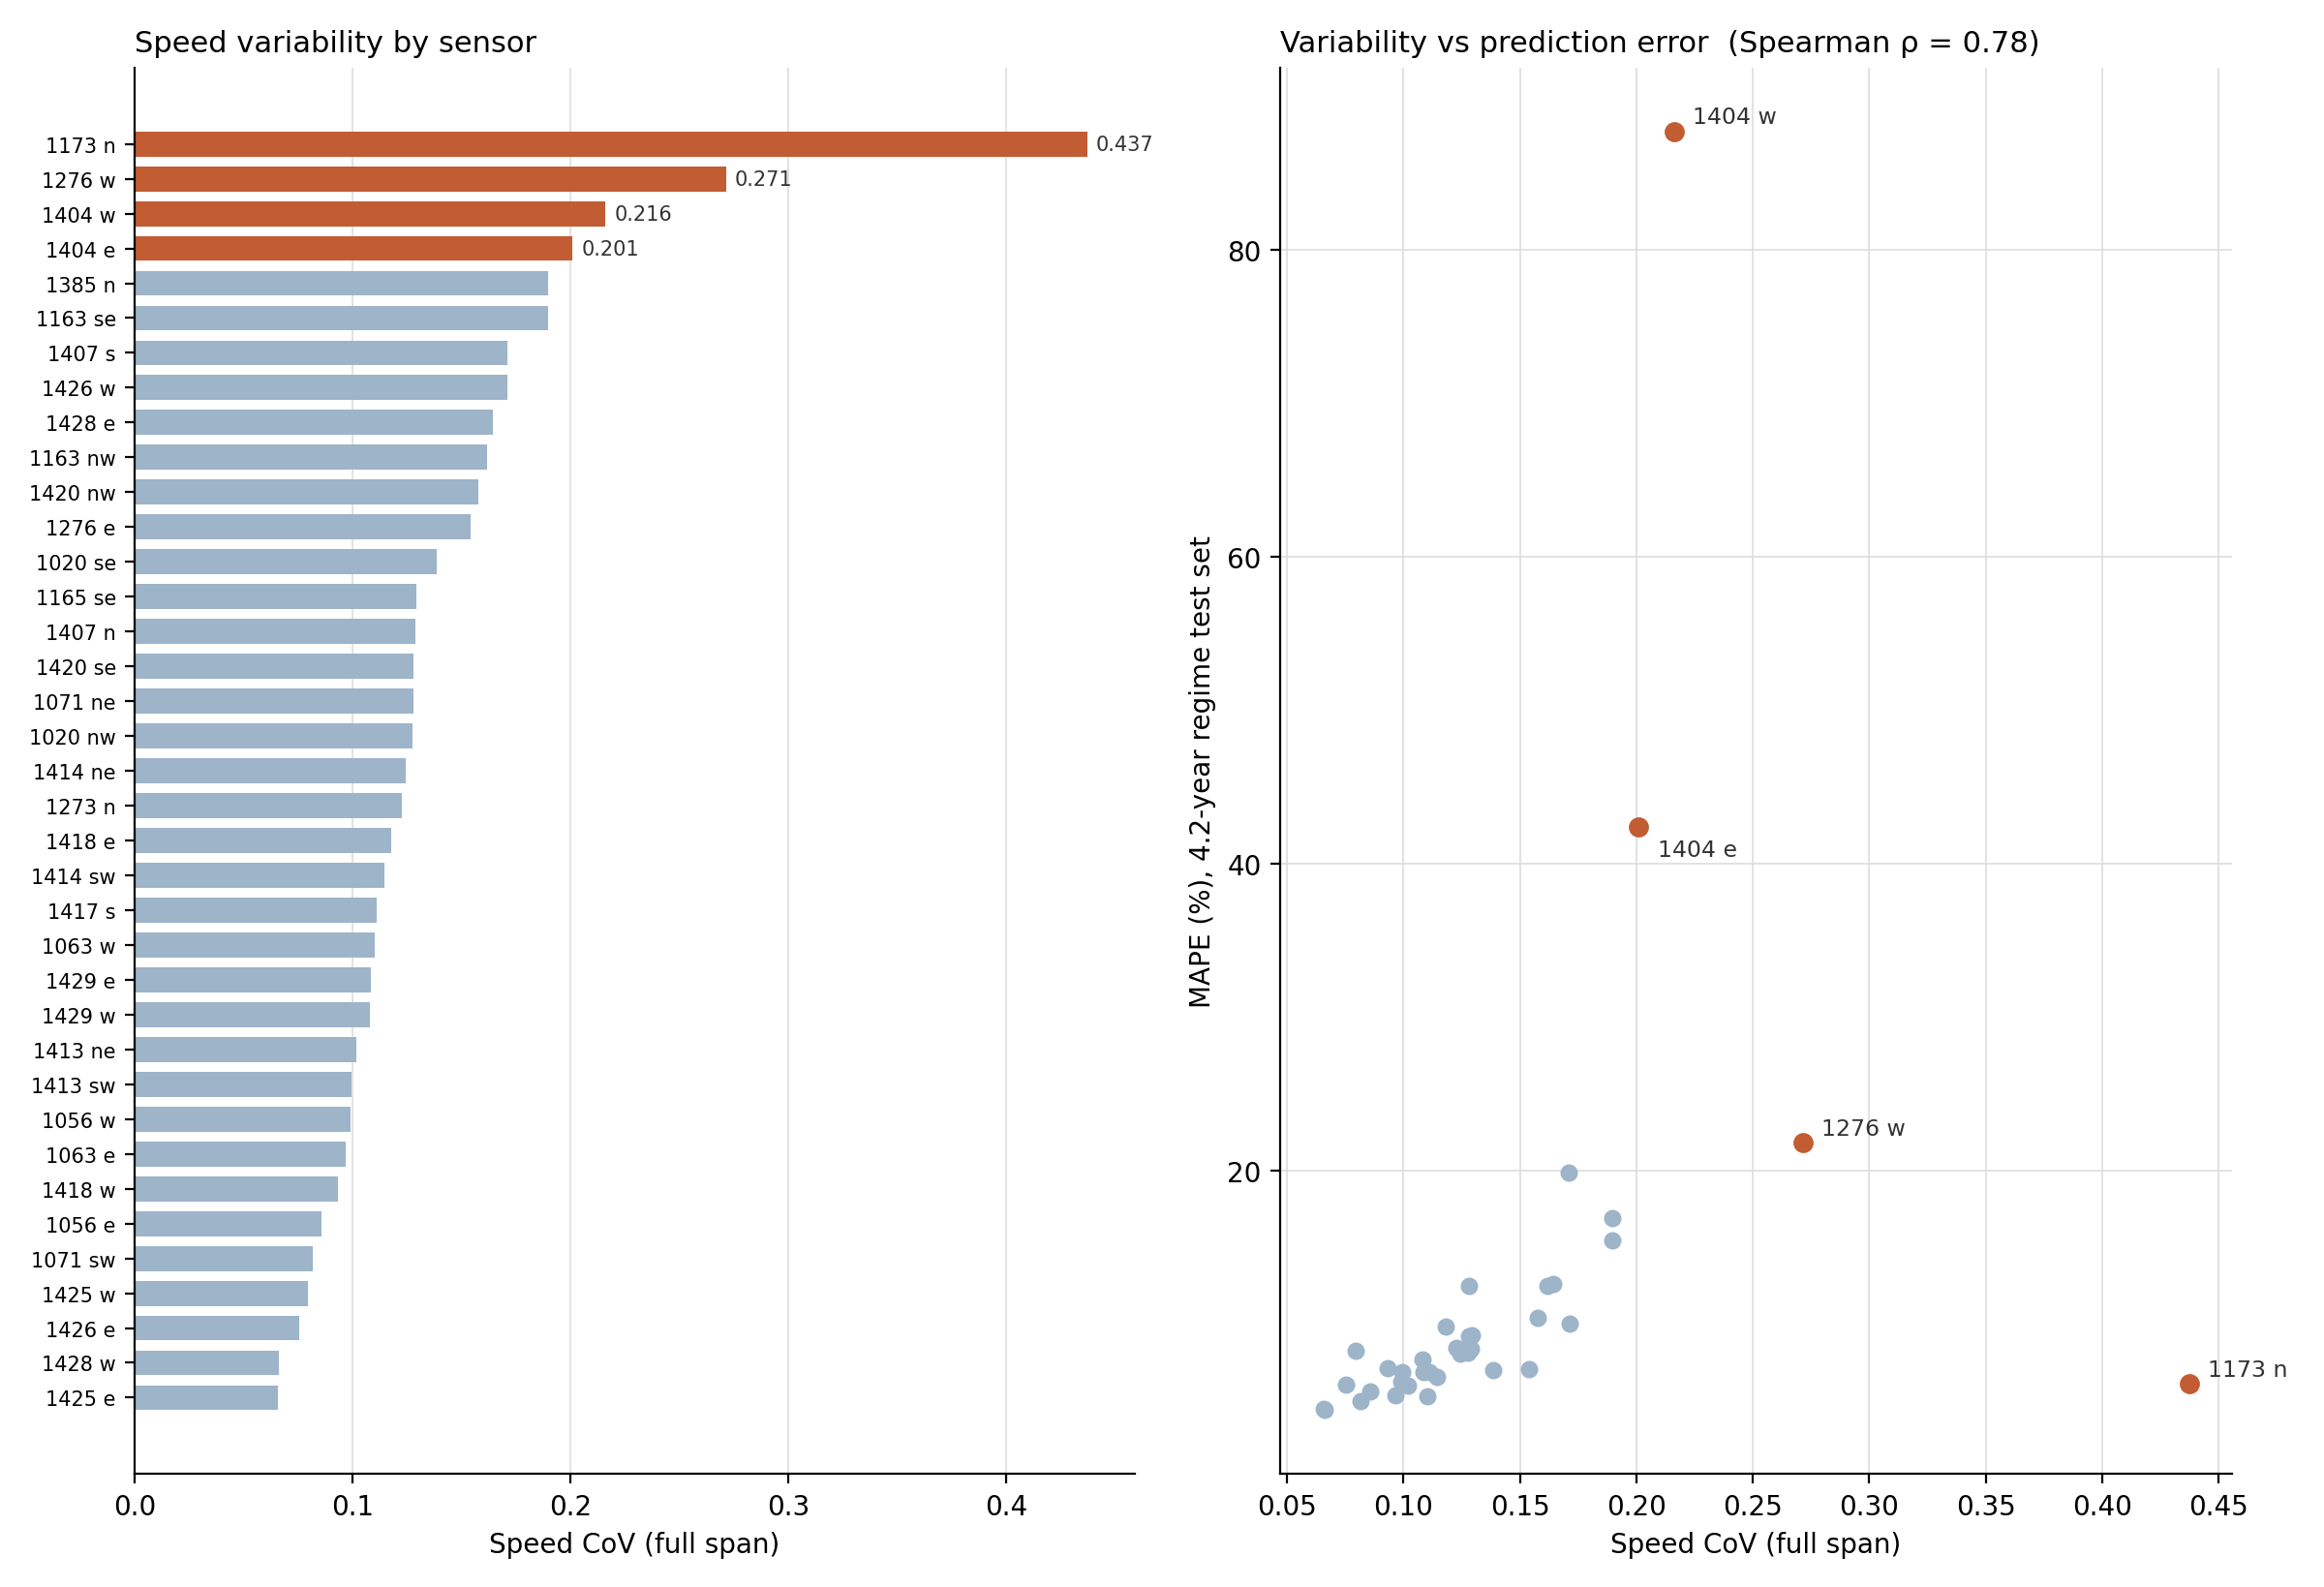
\includegraphics{speed_cov_mape.png}
\caption{Left: Speed CoV (full data span) per sensor, sorted; highlighted bars are the sensors discussed in the text. Right: Speed CoV against held-out MAPE under the 4.2-year regime (Spearman rho = 0.79). The two 1404 directions lie far above the trend: their error is driven by major traffic changes during the test period, not by intrinsic variability; 1173 north lies far below it, its CoV inflated by a historical level shift the model can absorb.}
\end{figure}

The figure below directly shows the day-to-day variability mechanism. With all weeks of full data span folded onto one Monday-Sunday axis, 1276 west's percentile band balloons through every daytime: the same clock time spans near-standstill to free flow depending on the week, so a calendar-feature model (which must predict a single value per slot) is bounded by that band width (a time-of-week average alone still leaves 22\% MAPE there). On 1425 east, the narrow ribbon explains its 4.5\% MAPE. The 1173 north band (middle panel) is the widest of the three, but for a different reason than 1276 west's, as it mixes weeks from only slightly different level regimes, mean speeds of 8-14 km/h in 2020-2021 versus \textasciitilde46 km/h thereafter. But because the level is stable within any given year, the model's year feature can track it, and the sensor remains well-predicted (with a 6.1\% MAPE). In short, for stable sites, prediction difficulty is driven by day-to-day spread at the same time of week, not by variability accumulated across years.

\begin{figure}
\centering
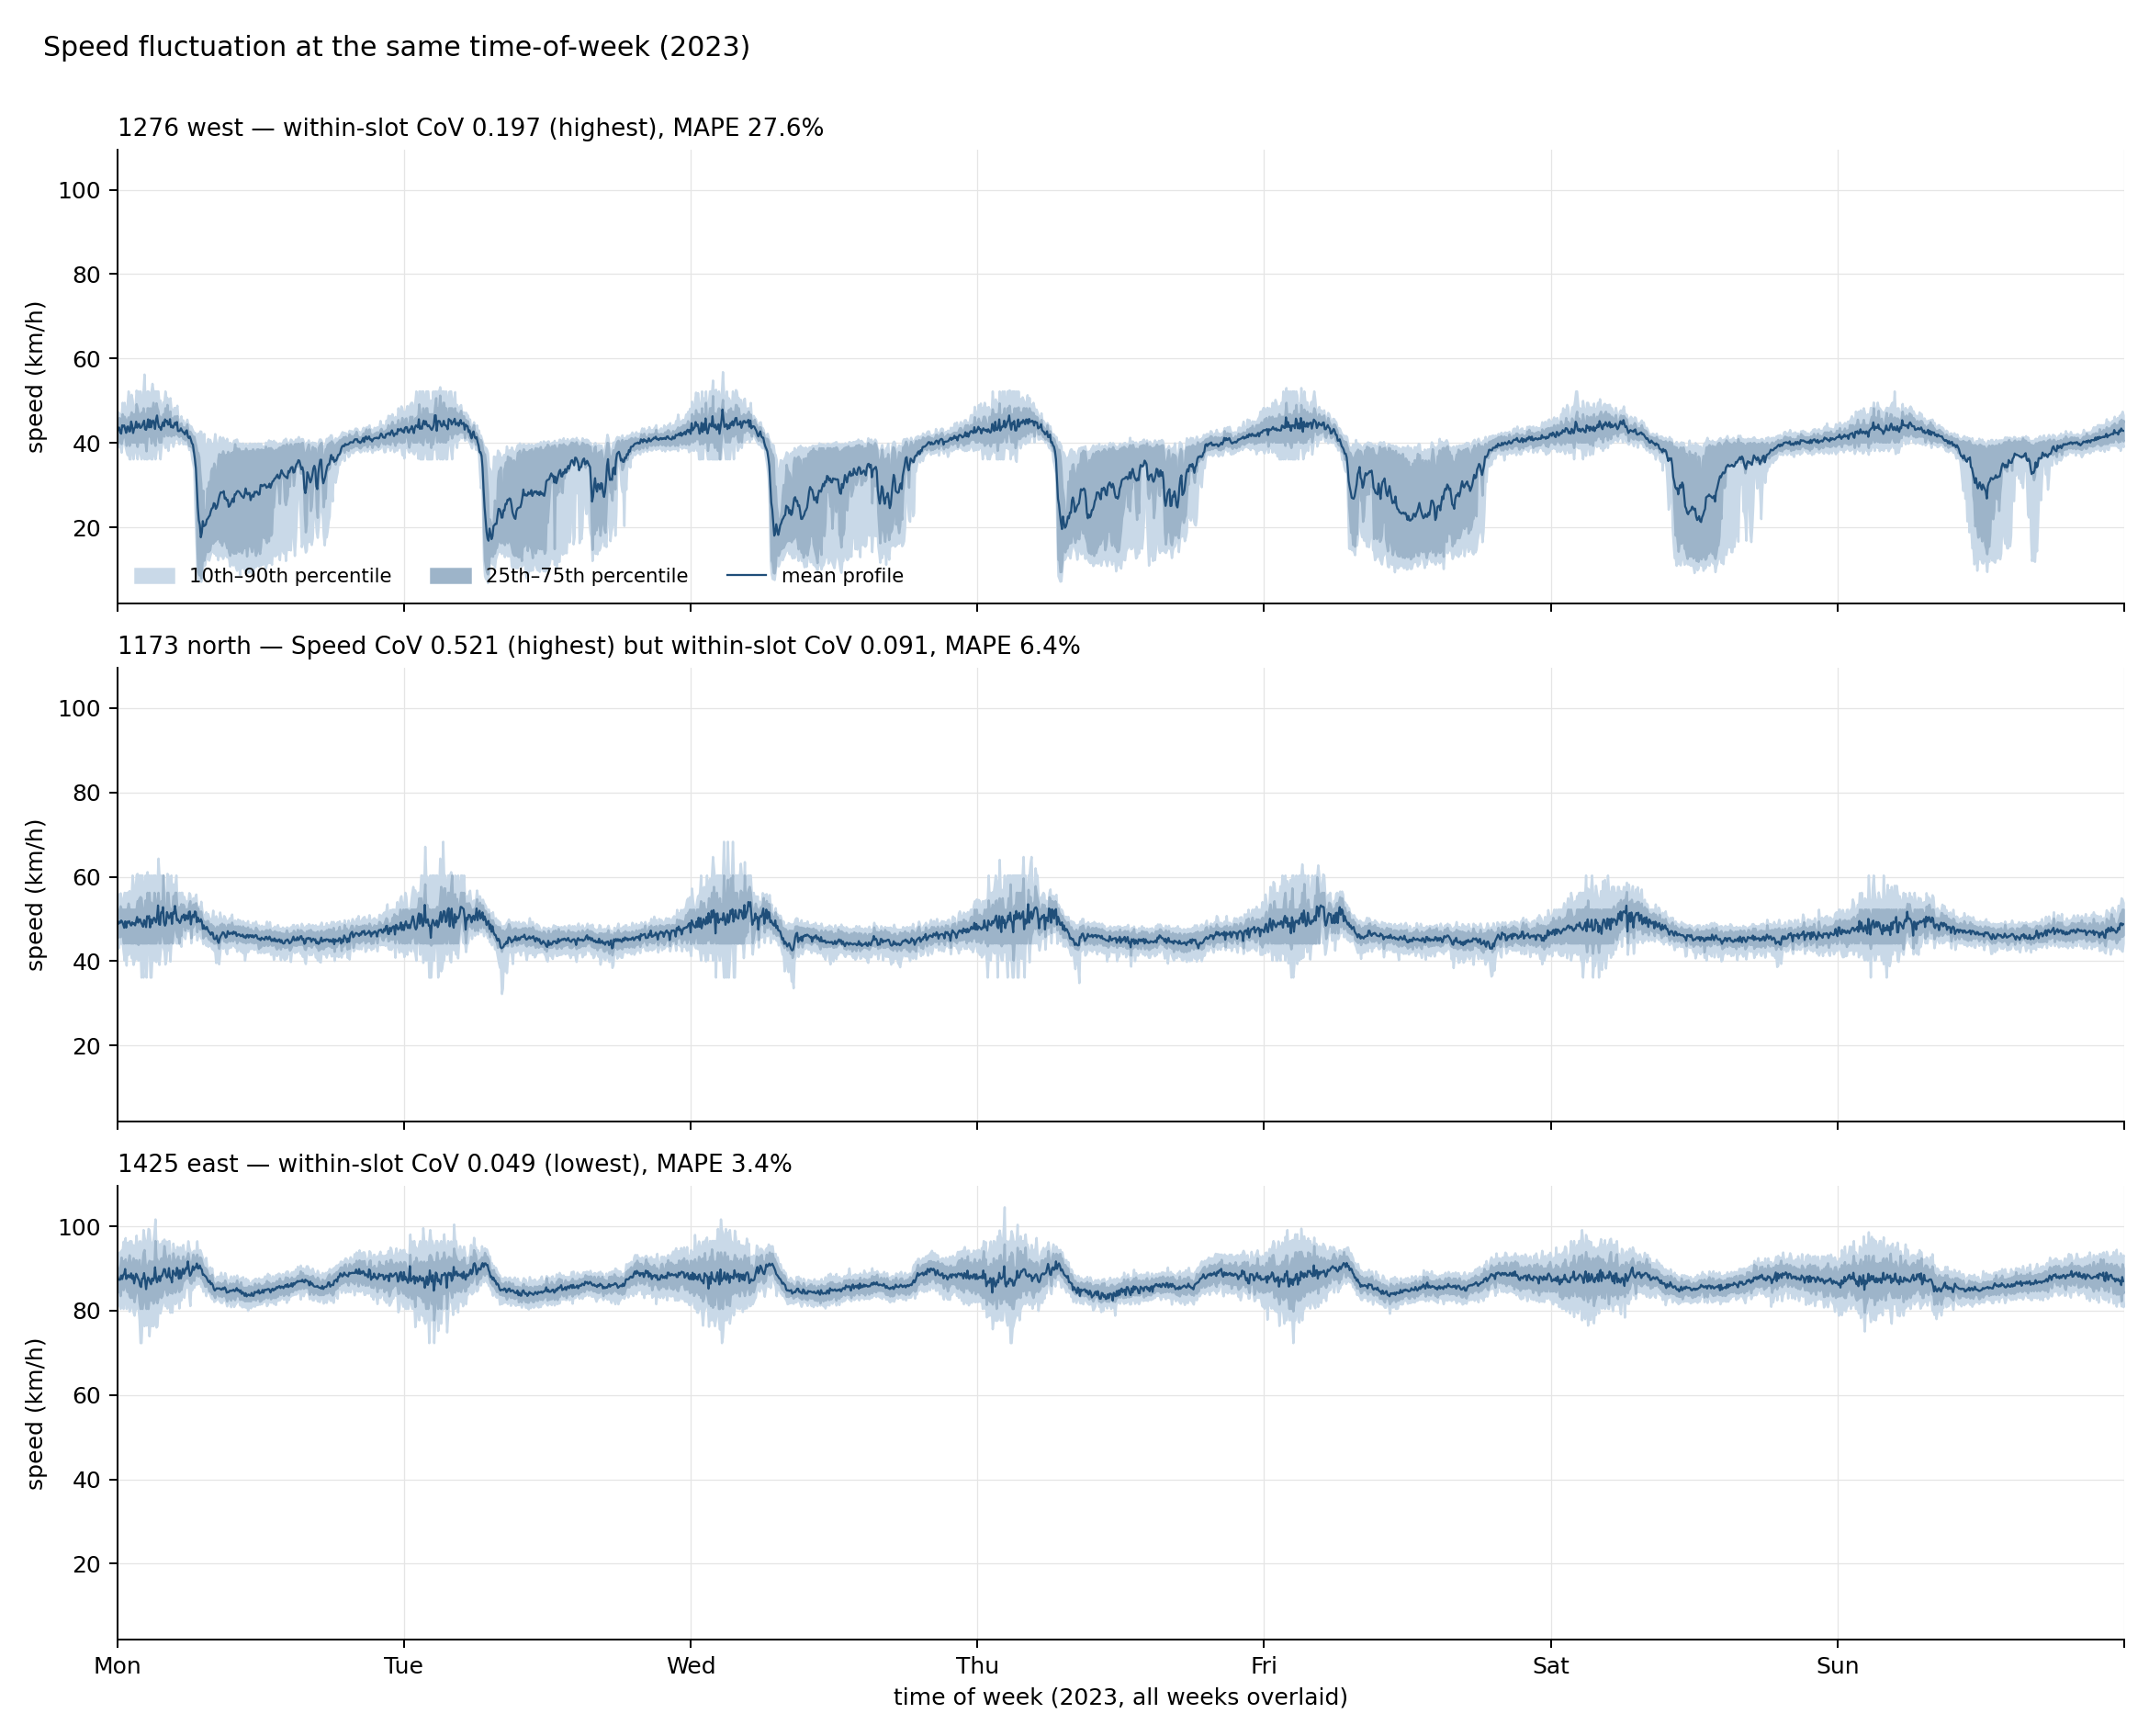
\includegraphics{sensor_1276w_profile.png}
\caption{Speed at the same time of week, all weeks of the full data span (Dec 2020 - Feb 2025) folded onto one Monday-Sunday axis at 5-minute resolution. At each slot, the line is the mean across all weeks, and the bands are the 25th-75th and 10th-90th percentiles of those same weeks. On 1276 west (top) the same clock time spans near-standstill to free flow depending on the week - genuine day-to-day unpredictability. On 1173 north (middle) the very wide band instead reflects weeks from different level regimes overlapping (the 2020-2021 low-speed period versus \textasciitilde46 km/h thereafter); this is what makes its Speed CoV the highest in the corpus while the sensor itself stays well predicted. On 1425 east (bottom) the narrow ribbon marks a road that barely varies at all. A calendar-feature model predicts one value per slot for a given date, so within-regime band width bounds its achievable accuracy.}
\end{figure}

The 1404 case is different, indicating site-level changes that cause significant traffic shifts. Their held-out test period (April 2024 - February 2025) contains a months-long degradation of the road itself: both directions slowed progressively from \textasciitilde57 km/h (August 2024) to \textasciitilde33 km/h (January 2025) with the monthly standard deviation rising from \textasciitilde5 to 17-23 km/h (most likely due to long-term site-level changes or road alteration at the site) so models trained on the earlier road are evaluated against a changed one. Independent traffic-count data from the same platform confirms the physical nature of the change, as monthly vehicle counts, stable for two years prior, then fall by roughly 30\% in November 2024 and by half from December 2024 in both directions (figure below, third panel). Since counts and speeds are separately measured quantities, their simultaneous collapse rules out a speed-sensor artefact. Recurrent December dips are visible in earlier years too (2021-2023) but recovered each January; however, the 2024-2025 episode differs in onset (September, months before the seasonal dip), depth (10th-percentile speeds near-standstill), and persistence (no January recovery by the end of the data) causing the very high MAPE of 1404 sensors. Excluding the two 1404 sensor directions, the aggregate MAPE of the remaining 35 sensors is 8.95\% (median 7.62\%).

\begin{figure}
\centering
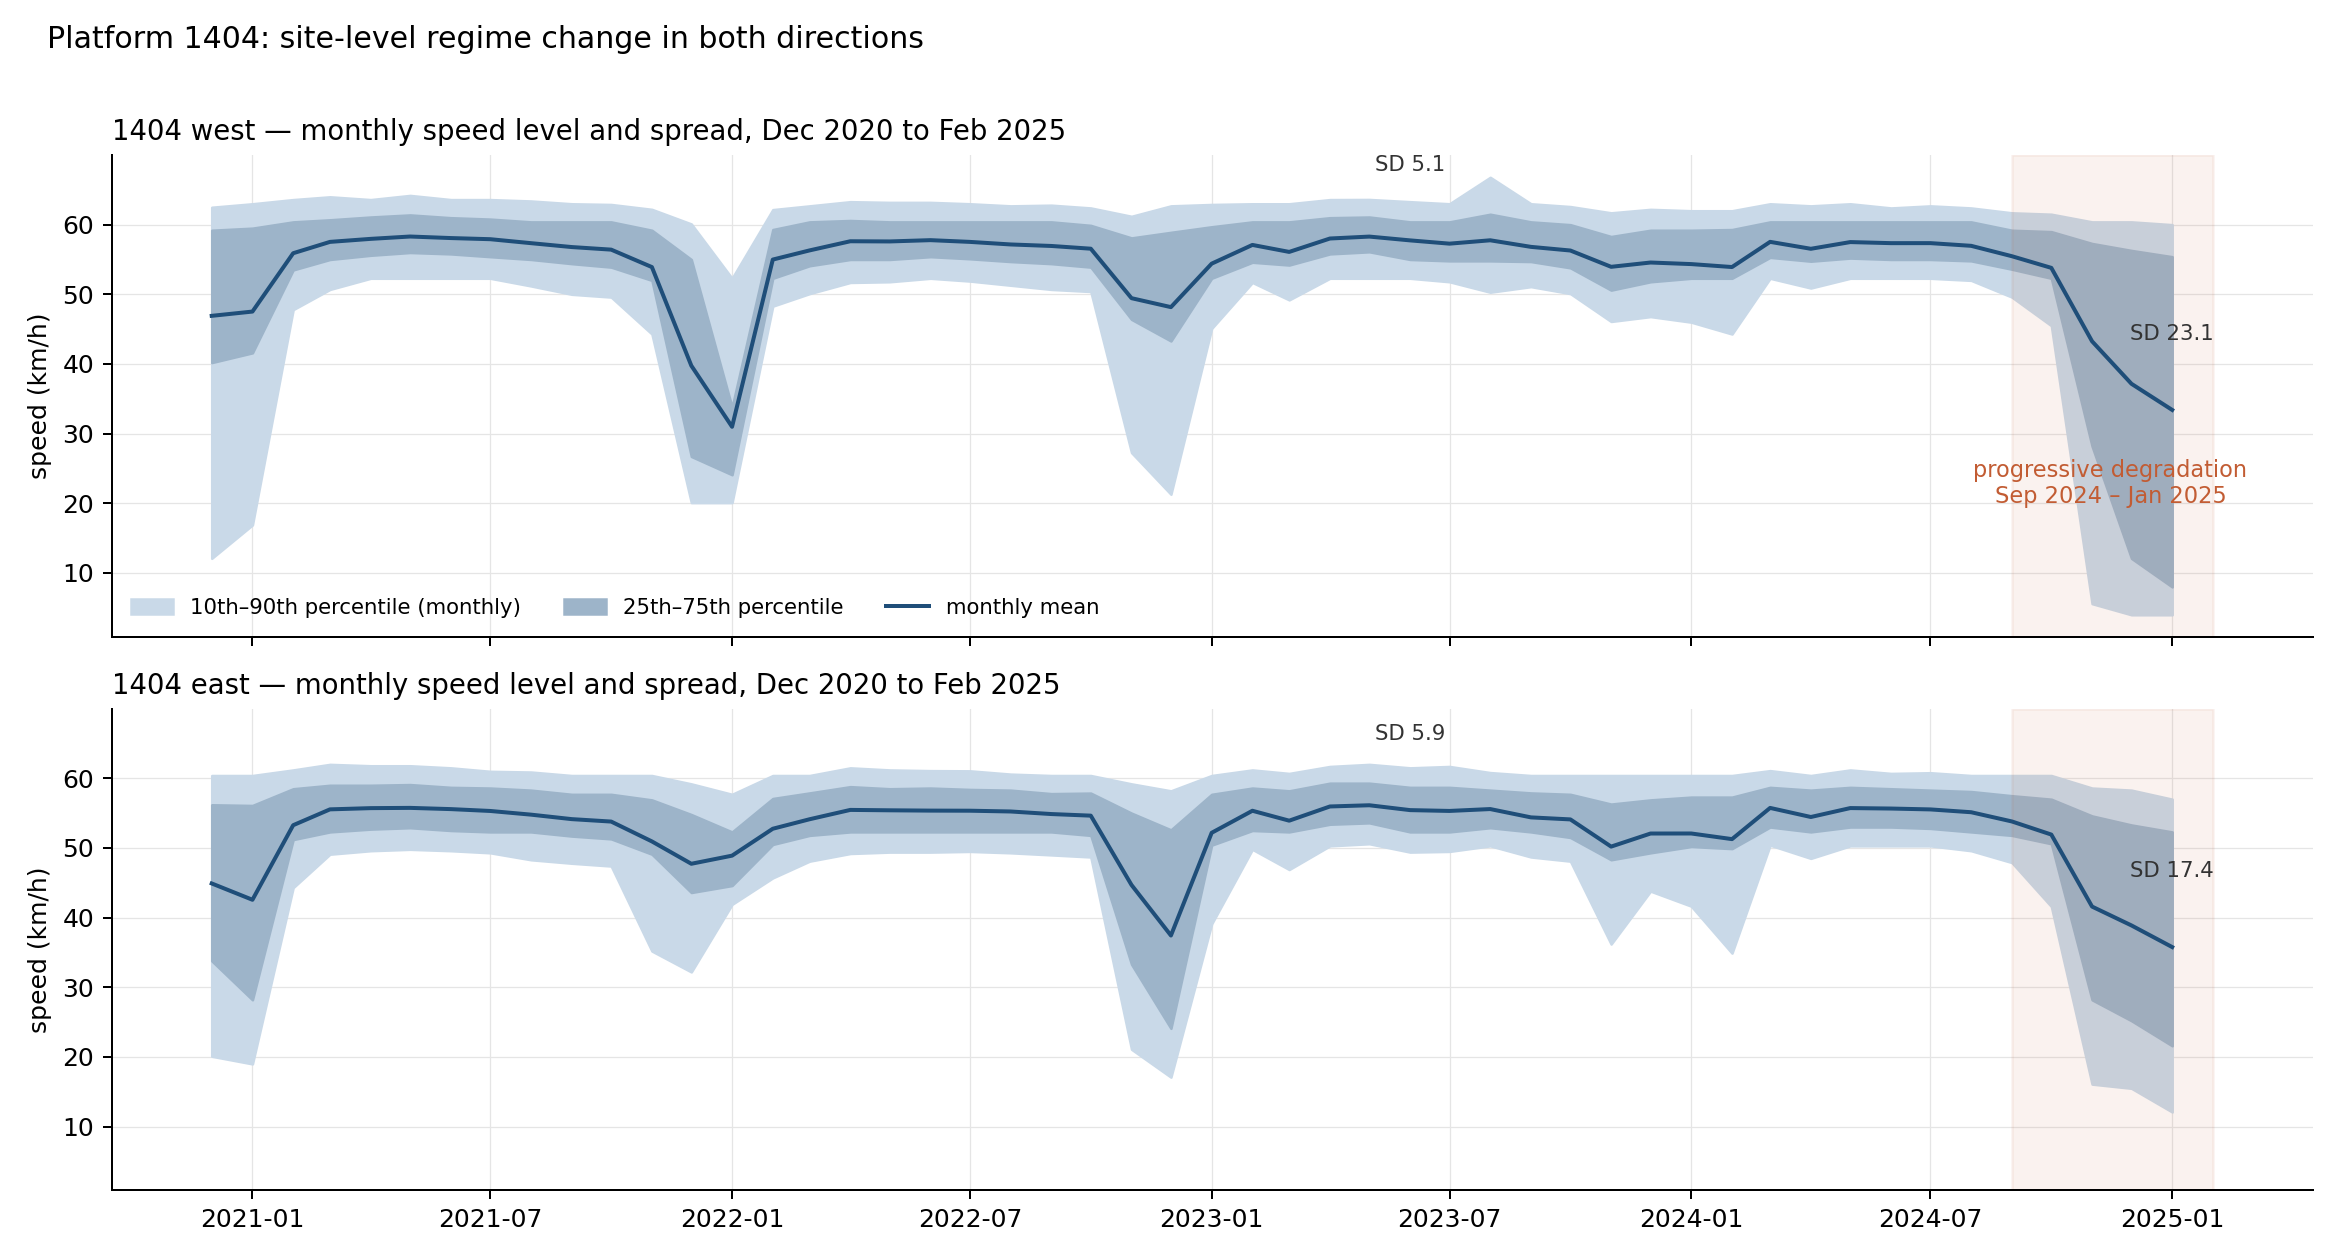
\includegraphics{sensor_1404_regime.png}
\caption{Platform 1404, three aligned views over the full span (Dec 2020 - Feb 2025). Top two panels: monthly mean speed with 25th-75th and 10th-90th percentile bands per direction (west: blue; east: green), each overlaid with the monthly MAPE of the 4.2-year models on the held-out months (orange dashed, right axis). The site was among the better-predicted locations before the disruption (6-8\% MAPE through summer 2024); error then rises with the site change to 364\% (west) and 148\% (east) by January 2025, exactly as the speed bands collapse. Bottom panel: independent monthly vehicle counts (all classes, both directions), stable at roughly 165,000-190,000 per direction until October 2024, then falling by about 30\% in November and roughly half from December - corroborating a major physical traffic alteration at the site rather than a sensor artefact.}
\end{figure}

The same site-level check was applied to the remaining highlighted high-MAPE sensors (figure below). None shows a December-2024 seasonal anomaly. One further site event was found: 1426 west is stable at \textasciitilde80 km/h until December 2024 and then drops to 62 km/h in January 2025, with its monthly standard deviation tripling to \textasciitilde27 km/h - a late-onset disruption inside the final month of the test period, which partially accounts for its 19.9\% MAPE. The other three behave as their variability columns predict: 1276 west and 1163 southeast hold stable levels throughout (their errors are intrinsic day-to-day spread), and 1385 north shows only a modest level rise (\textasciitilde37 to \textasciitilde41 km/h) from August 2024. Errors at the highlighted sensors therefore divide into two classes: intrinsic day-to-day variability (1276 west, 1163 southeast, 1385 north) and site changes during the test period (1404 both directions, and 1426 west in its final month).

\begin{figure}
\centering
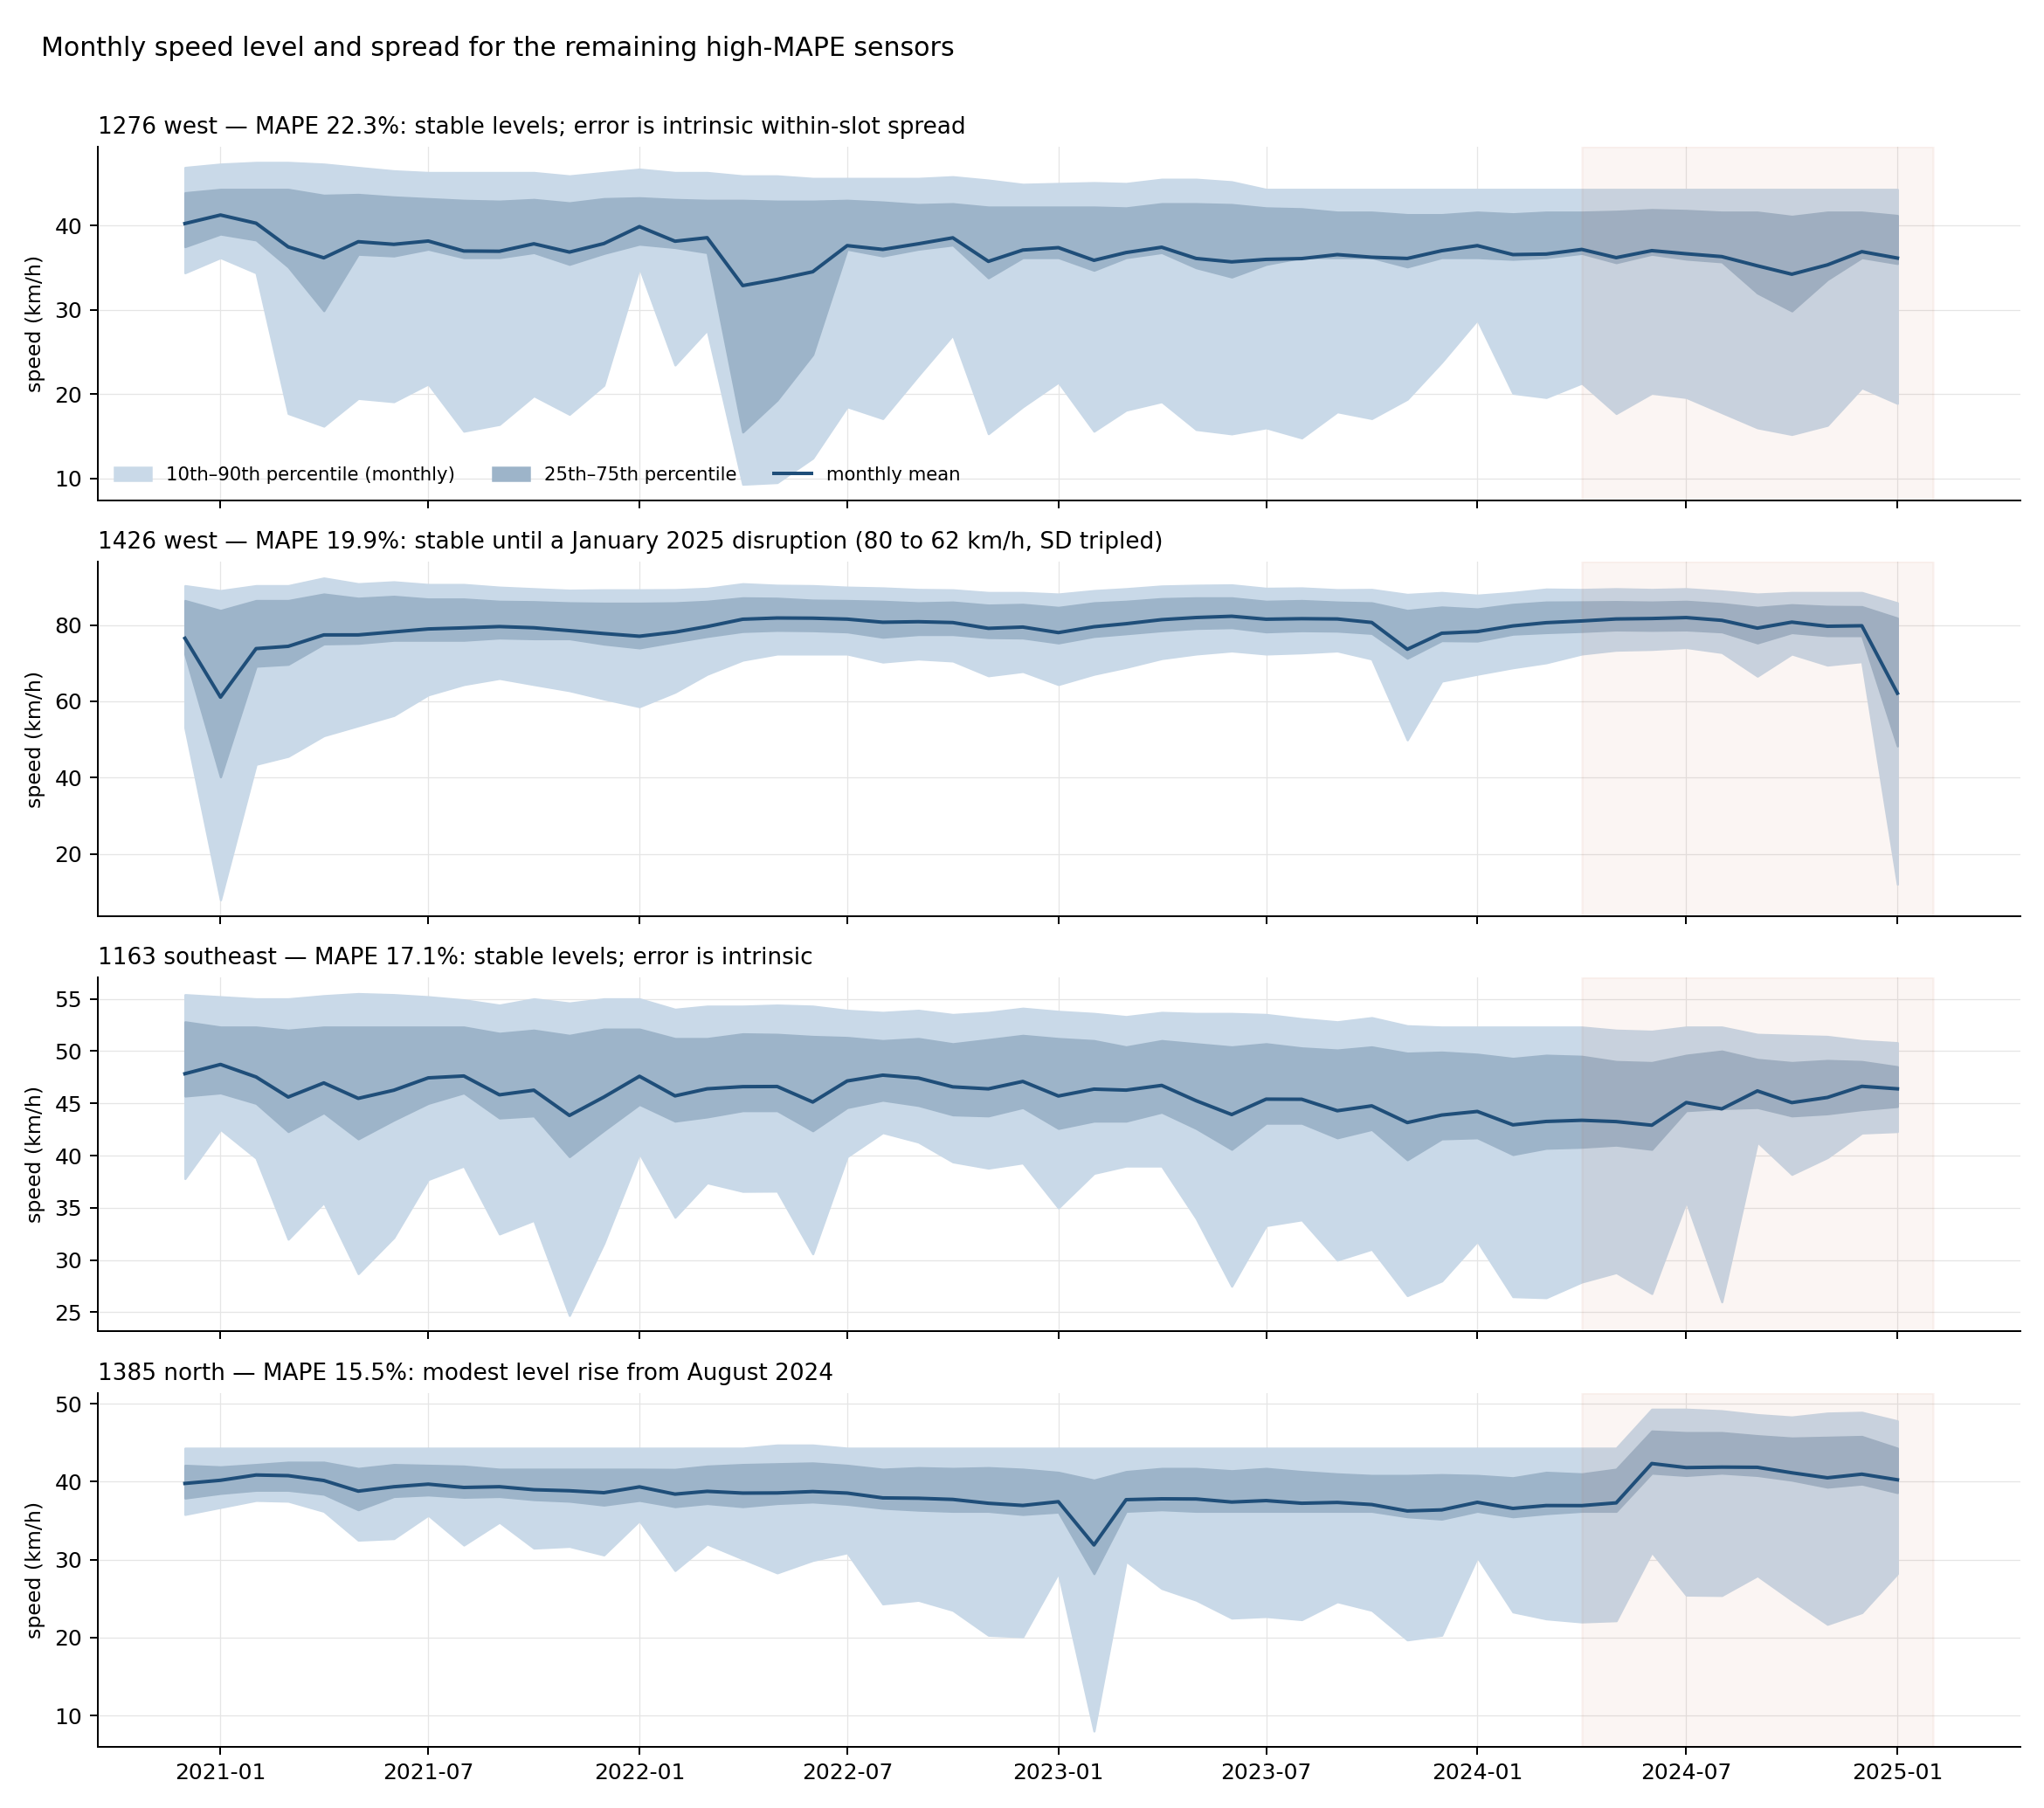
\includegraphics{sensor_highmape_monthly.png}
\caption{Monthly speed level and spread for the remaining high-MAPE sensors over the full span; the shaded region is the held-out test period (April 2024 - February 2025). 1426 west shows a January 2025 disruption; 1276 west, 1163 southeast, and 1385 north show no site-level change.}
\end{figure}

\hypertarget{common-test-set-scenario-comparison}{%
\subsection{Common-test-set scenario comparison for re-training evaluation}\label{common-test-set-scenario-comparison}}

\hypertarget{why-a-common-test-set}{%
\subsubsection{Why a common test set for re-training evaluation?}\label{why-a-common-test-set}}

In our original protocol, each training scenario was evaluated on the final 20\% of its own data range. Because the re-training scenarios cover different date ranges, each was therefore tested on a different slice of calendar time: the 3-year base on roughly mid-2023 to December 2023, the 4.2-year cold start on April 2024 to February 2025, and each re-training window on the final weeks of its own update period. A comparison built on those numbers mixes two things we cannot separate: how good each model is, and how difficult its particular test slice happened to be. Calendar periods genuinely differ in difficulty (seasonal traffic, holiday effects, and site events such as the platform 1404 degradation make late 2024 substantially harder than late 2023) so a scenario could score worse simply because it sat a harder exam.

We therefore re-evaluated the already-trained models of every scenario, frozen, on three identical held-out periods that none of them trained on: a two-month window (1 December 2024 to 1 February 2025), a four-month window (1 October 2024 to 1 February 2025), and a nine-month window (1 May 2024 to 1 February 2025). Same sensors, same weeks, same conditions for all scenarios; any remaining difference in error can only come from the models themselves. One rule keeps this fair in the other direction as well: a scenario is excluded from any window that overlaps its own training data, which is why PW12 (trained to September 2024) does not appear in the nine-month column.

This correction changed our conclusions materially. The apparent advantage of the 3-year base over the 4.2-year cold start reversed: on every common window the cold start is better, and the earlier pattern reflected only that the base model's private test slice (2023) was easier than the cold start's (2024-2025). The apparent degradation of the tiny tier under longer re-training windows dissolved for the same reason. The central re-training result survived, at roughly one MAPE point rather than the two to five points implied by window-local evaluation - real, but smaller than the original protocol made it look.

All training scenarios in the paper (3-year base, 4.2-year cold start, and progressive warm-start retraining windows PW3/PW6/PW12) were additionally evaluated over identical held-out periods. Each cell reports mean MAE (mph) / mean MAPE (\%) / median MAPE (\%):

\begin{longtable}[]{@{}llll@{}}
\toprule
\begin{minipage}[b]{0.22\columnwidth}\raggedright
Scenario\strut
\end{minipage} & \begin{minipage}[b]{0.22\columnwidth}\raggedright
Dec 2024 - Feb 2025\strut
\end{minipage} & \begin{minipage}[b]{0.22\columnwidth}\raggedright
Oct 2024 - Feb 2025\strut
\end{minipage} & \begin{minipage}[b]{0.22\columnwidth}\raggedright
May 2024 - Feb 2025\strut
\end{minipage}\tabularnewline
\midrule
\endhead
\begin{minipage}[t]{0.22\columnwidth}\raggedright
base (3y)\strut
\end{minipage} & \begin{minipage}[t]{0.22\columnwidth}\raggedright
3.09 / 19.09 / 8.89\strut
\end{minipage} & \begin{minipage}[t]{0.22\columnwidth}\raggedright
2.83 / 16.51 / 9.23\strut
\end{minipage} & \begin{minipage}[t]{0.22\columnwidth}\raggedright
2.44 / 12.25 / 7.84\strut
\end{minipage}\tabularnewline
\begin{minipage}[t]{0.22\columnwidth}\raggedright
cold start (4.2y)\strut
\end{minipage} & \begin{minipage}[t]{0.22\columnwidth}\raggedright
3.02 / 22.88 / 9.07\strut
\end{minipage} & \begin{minipage}[t]{0.22\columnwidth}\raggedright
2.71 / 18.03 / 8.76\strut
\end{minipage} & \begin{minipage}[t]{0.22\columnwidth}\raggedright
2.32 / 12.49 / 8.07\strut
\end{minipage}\tabularnewline
\begin{minipage}[t]{0.22\columnwidth}\raggedright
re-train PW3\strut
\end{minipage} & \begin{minipage}[t]{0.22\columnwidth}\raggedright
2.91 / 22.16 / 8.78\strut
\end{minipage} & \begin{minipage}[t]{0.22\columnwidth}\raggedright
2.68 / 17.78 / 8.18\strut
\end{minipage} & \begin{minipage}[t]{0.22\columnwidth}\raggedright
2.35 / 12.52 / 7.48\strut
\end{minipage}\tabularnewline
\begin{minipage}[t]{0.22\columnwidth}\raggedright
re-train PW6\strut
\end{minipage} & \begin{minipage}[t]{0.22\columnwidth}\raggedright
2.89 / 21.85 / 8.33\strut
\end{minipage} & \begin{minipage}[t]{0.22\columnwidth}\raggedright
2.64 / 17.55 / 8.32\strut
\end{minipage} & \begin{minipage}[t]{0.22\columnwidth}\raggedright
2.31 / 12.31 / 7.59\strut
\end{minipage}\tabularnewline
\begin{minipage}[t]{0.22\columnwidth}\raggedright
re-train PW12\strut
\end{minipage} & \begin{minipage}[t]{0.22\columnwidth}\raggedright
2.90 / 21.97 / 8.44\strut
\end{minipage} & \begin{minipage}[t]{0.22\columnwidth}\raggedright
2.61 / 17.46 / 7.71\strut
\end{minipage} & \begin{minipage}[t]{0.22\columnwidth}\raggedright
excluded*\strut
\end{minipage}\tabularnewline
\bottomrule
\end{longtable}

*PW12 trains up to September 2024, overlapping the nine-month window.

The two accuracy metrics disagree here, and the disagreement is informative: these evaluation windows fall inside the platform-1404 degradation period, and the two 1404 directions dominate the mean MAPE (raising it to 12-23\% and making the 3-year base appear best on that metric even though it is worst on MAE in every window). Median MAPE, which reflects the typical sensor, stays at 7.5-9.2\% across all scenarios and broadly preserves the ordering of MAE. Scenario rankings should therefore be read from the MAE column; on it, warm-start re-training improves on both cold-start baselines in every window.

Prediction accuracy is invariant to the training platform (across repeated runs and platforms, the standard deviation of aggregate MAPE is below 0.3 percentage points in over 90\% of measured cells).

\hypertarget{measurement-imprecision-repeated-runs}{%
\subsection{Measurement imprecision (repeated
runs)}\label{measurement-imprecision-repeated-runs}}

Wall-clock training times are subject to run-to-run variation; every reported configuration was therefore executed repeatedly, at least five times for the training scenarios tabulated below, and at least three times for the re-training grid and is summarised as mean, standard deviation (SD), and a 95\% confidence interval (Student's t). The table lists the training scenarios for every platform and sensor tier.

The number of runs varies across cells for three reasons. (1) Repetition was allocated differentially: short or high-variance configurations were repeated at least five times, while multi-hour configurations were kept at three repeats once their observed CoV was below \textasciitilde4\%, following standard practice in performance evaluation. (2) Cells pool every clean batch of the same configuration across measurement campaigns (February, March, and September 2026), so frequently exercised configurations accumulated more runs (e.g.~n = 8-9 for the fog and cloud training cells). (3) The Dell cells come exclusively from a campaign on verified mains power, after telemetry showed that runs from an earlier campaign had intermittently executed in an OS power-capped state.

\begin{longtable}[]{@{}llllllll@{}}
\toprule
Platform & Scenario & Tier & n & Mean (s) & SD (s) & 95\% CI half-width (s) & CoV (\%)\tabularnewline
\midrule
\endhead
CSF3 Cloud GPU (A100) & initial (3y) & tiny & 5 & 61.2 & 12.6 & 15.7 &
20.6\tabularnewline
CSF3 Cloud GPU (A100) & initial (3y) & small & 5 & 604.0 & 33.4 & 41.5 &
5.5\tabularnewline
CSF3 Cloud GPU (A100) & initial (3y) & medium & 5 & 1,609.8 & 25.8 &
32.1 & 1.6\tabularnewline CSF3 Cloud GPU (A100) & initial (3y) & full & 5 & 2,153.9 & 34.8 & 43.3
& 1.6\tabularnewline
CSF3 Cloud GPU (A100) & cold start (4.2y) & tiny & 7 & 66.2 & 14.7 &
13.6 & 22.2\tabularnewline
CSF3 Cloud GPU (A100) & cold start (4.2y) & small & 9 & 690.6 & 39.2 &
30.1 & 5.7\tabularnewline CSF3 Cloud GPU (A100) & cold start (4.2y) & medium & 9 & 1,861.5 & 79.6
& 61.3 & 4.3\tabularnewline
CSF3 Cloud GPU (A100) & cold start (4.2y) & full & 9 & 2,461.0 & 123.4 &
95.0 & 5.0\tabularnewline
Dell Precision Fog GPU & initial (3y) & tiny & 5 & 43.3 & 5.0 & 6.2 &
11.5\tabularnewline
Dell Precision Fog GPU & initial (3y) & small & 5 & 490.7 & 5.0 & 6.2 &
1.0\tabularnewline
Dell Precision Fog GPU & initial (3y) & medium & 5 & 1,286.6 & 40.9 &
50.8 & 3.2\tabularnewline Dell Precision Fog GPU & initial (3y) & full & 5 & 1,723.8 & 33.4 & 41.5
& 1.9\tabularnewline
Dell Precision Fog GPU & cold start (4.2y) & tiny & 5 & 46.7 & 7.7 & 9.6
& 16.5\tabularnewline
Dell Precision Fog GPU & cold start (4.2y) & small & 5 & 507.8 & 22.7 &
28.3 & 4.5\tabularnewline Dell Precision Fog GPU & cold start (4.2y) & medium & 5 & 1,376.4 & 28.3
& 35.1 & 2.1\tabularnewline
Dell Precision Fog GPU & cold start (4.2y) & full & 5 & 1,865.8 & 44.9 &
55.9 & 2.4\tabularnewline
CSF3 Jetson Sim & initial (3y) & tiny & 5 & 72.8 & 22.2 & 27.6 &
30.4\tabularnewline
CSF3 Jetson Sim & initial (3y) & small & 5 & 730.6 & 42.0 & 52.2 &
5.8\tabularnewline
CSF3 Jetson Sim & cold start (4.2y) & tiny & 6 & 66.1 & 11.2 & 11.8 &
17.0\tabularnewline
CSF3 Jetson Sim & cold start (4.2y) & small & 6 & 683.6 & 38.0 & 39.8 &
5.6\tabularnewline
CSF3 Edge RSU Sim & initial (3y) & tiny & 5 & 151.5 & 28.6 & 35.6 &
18.9\tabularnewline
CSF3 Edge RSU Sim & initial (3y) & small & 5 & 1,737.7 & 156.9 & 195.0 &
9.0\tabularnewline
CSF3 Edge RSU Sim & cold start (4.2y) & tiny & 8 & 120.1 & 39.8 & 33.2 &
33.1\tabularnewline
CSF3 Edge RSU Sim & cold start (4.2y) & small & 6 & 1,342.5 & 254.5 &
267.0 & 19.0\tabularnewline
CSF3 RPi Sim & initial (3y) & tiny & 5 & 133.1 & 32.7 & 40.7 &
24.6\tabularnewline
CSF3 RPi Sim & initial (3y) & small & 5 & 1,692.7 & 162.4 & 201.8 &
9.6\tabularnewline
CSF3 RPi Sim & cold start (4.2y) & tiny & 8 & 132.3 & 20.6 & 17.2 &
15.5\tabularnewline
CSF3 RPi Sim & cold start (4.2y) & small & 6 & 1,572.2 & 177.5 & 186.2 &
11.3\tabularnewline
AWS t2.medium RSU & initial (3y) & tiny & 5 & 159.9 & 10.8 & 13.5 &
6.8\tabularnewline
AWS t2.medium RSU & initial (3y) & small & 5 & 2,649.1 & 1,519.6 &
1,889.2 & 57.4\tabularnewline AWS t2.medium RSU & cold start (4.2y) & tiny & 10 & 160.9 & 37.9 & 27.1
& 23.5\tabularnewline
AWS t2.medium RSU & cold start (4.2y) & small & 6 & 2,760.6 & 1,451.1 &
1,522.5 & 52.6\tabularnewline
\bottomrule
\end{longtable}

The warm-start re-training configurations (six windows x four tiers on the fog and Jetson-simulation platforms, plus three progressive windows on AWS) were run n = 2-6 times each; their median CoV is 3.6\%. Two systematic variance mechanisms were identified from run telemetry and are reported as findings rather than averaged away: OS power-state frequency capping on the fog workstation (affected runs excluded by the stated rule) and burstable CPU-credit exhaustion on the AWS t2.medium, whose initial small-tier cell is bimodal - approximately 1,970 +/- 160 s with credits available versus \textasciitilde5,360 s when exhausted - which is why its pooled SD is large.

Prediction accuracy, by contrast, is essentially noiseless across repetitions and platforms: over all repeated cells, the across-run standard deviation of aggregate MAPE has a median of only 0.06 percentage points (90th percentile 0.27 pp), which therefore substantiates reporting a single accuracy figure per configuration while wall-clock times carry mean +/- SD.

\end{document}
